\section{Introduction}
\emph{XIST} and \emph{Rsx} provide compelling examples of how the sequence-to-function relationship in lncRNAs may be modular in nature \cite{Brockdorff2018LocalNcRNA, Sprague2019NonlinearDomains,Pintacuda2017HnRNPKSilencing,Wang2017TargetingGuanines,Zhao2008PolycombChromosome}. These two transcripts demonstrate clear sequence regions, defined by the boundaries of their tandem repeat domains \cite{Brown10TheNucleus.,Brockdorff10TheNucleus.,Sprague2019NonlinearDomains,Grant2012RsxInactivation}, that are conserved and are clearly functional as demonstrated by the binding of RNA binding proteins to their transcripts \cite{Hoki2009AMouse,Moindrot2015ASilencing,Sunwoo2017RepeatCIZ1,Nesterova2001CharacterizationSequence,Royce-Tolland2010TheInactivation,Brown10TheNucleus.,Brockdorff10TheNucleus.}. Our model of lncRNA function, specifically the bag-of-words model that the order of short motifs in a sequence is less important than their overall density \cite{Kirk2018FunctionalContent}, implicitly means that a tandem repeated sequence may not be essential for recruitment of these RNA binding proteins \cite{Sprague2019NonlinearDomains}.

It is possible to show that the $k$-mer content of a sequence can be perfectly preserved while destroying the tandomly repeated nature of a sequence (Fig \ref{fig:shufD} A-C). This can be done by building a graph whose nodes are $(k-1)$-mers and whose edges are connected such that a sequence is reconstructed with the exact same $k$-mer frequencies as the original sequence \cite{Jiang2008UShuffle:Counts}. Furthermore, if we examine lncRNA sequences in mouse with very high SEEKR correlation to HXD it is clear that not all these sequences contain substantial tandemly repeated sequence as in \emph{XIST} (Fig \ref{fig:shufD} D-H). 
\begin{figure}[h]
\centering
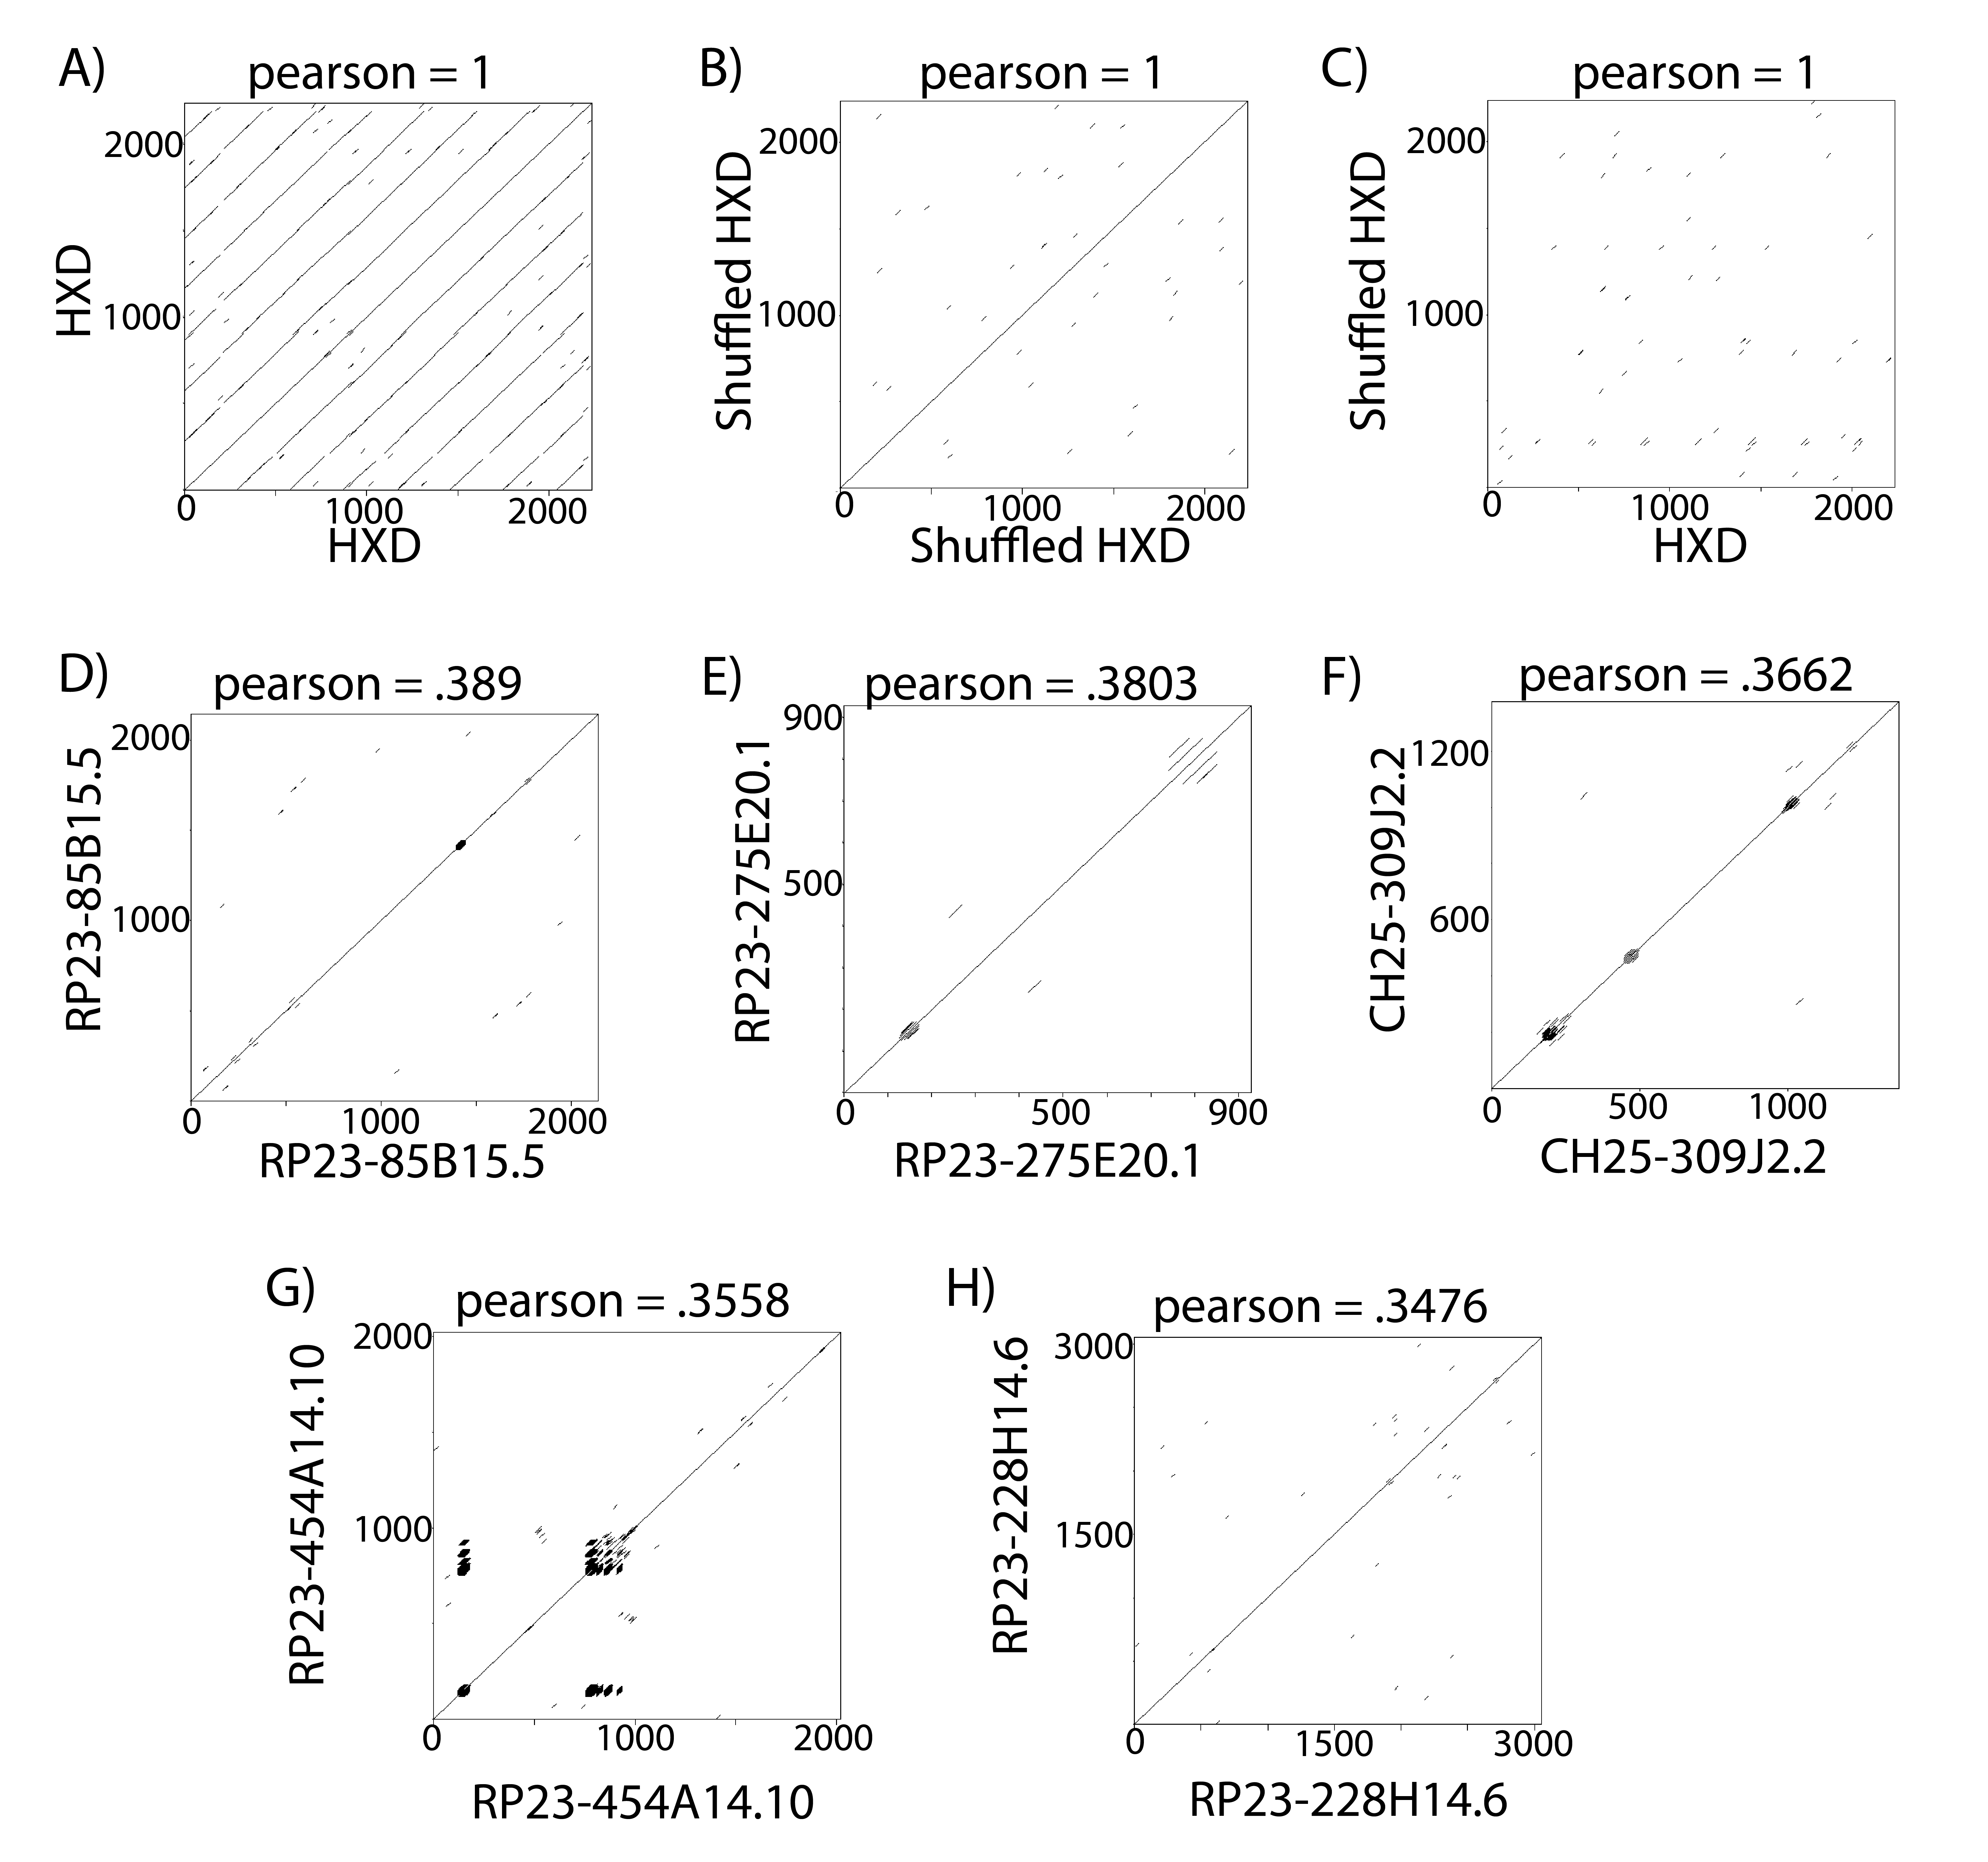
\includegraphics[width=\textwidth]{shufD.png}
\caption[Shuffling $k$-mers destroyed tandem repeat without changing motif content]{Dot plot alignments and SEEKR-defined similarity between human Xist Repeat D, shuffled Repeat D, and the top 5 mouse lncRNAs that are most similar to Repeat D. Repeat D was shuffled using $\mu$Shuffle and preserving $k$-mer content at $k$ = 4 (Jiang et al., 2008). Dotplots were generated using a window size 20 nucleotides and a threshold of 50\% identity.}
\label{fig:shufD}
\end{figure}

Therefore, a challenge in understanding lncRNA function is identifying where functional modules may be located within a sequence \cite{Pang2006RapidFunction,Hezroni2015PrinciplesSpecies,Johnson2014TheRNAs}. Clearly, the answer is not solely exonic sequence as in a protein coding reading frame. Within \emph{XIST} these sequence regions are sub-sequences within the spliced transcript \cite{Brockdorff10TheNucleus.,Brown10TheNucleus.,Brockdorff2018LocalNcRNA,Sprague2019NonlinearDomains,Pintacuda2017HnRNPKSilencing,Hoki2009AMouse,Sunwoo2017RepeatCIZ1}. Compounding the issue is that as far as is known, no specific boundary motifs (\emph{e.g.}, splice junction boundaries) are required. Potential splice junctions in genes are relatively easy to identify based off a combination of sequence content, and the presence of conserved 5' and 3' splice site motifs that demarcate the beginning and end of an intron, respectively \cite{Burge1997PredictionDNA}. 

To model this hypothesized sequence structure, we have developed an HMM that is designed to identify sub-sequences within a larger transcript that contain regions of elevated $k$-mer content to a known functional domain. Given how little is known in the field about the sequence-to-function relationship in lncRNAs, we use the archetypal lncRNA \emph{XIST} and its known functional sub-sequences (A-,B-,D-,E- repeats) as our model. 
\section{Results}
\subsection{Model Structure}
Given a transcript sequence, $X$, of length $L$, and a set of predefined functional features $Y$, the objective is to map each nucleotide $x \in X$ to a functional state, $y \in Y$. Our underlying biological hypothesis is that non-coding RNAs contain sub-sequences of specific $k$-mer content that is enriched for motifs that bind a specific RBP or subset of RBPs and that these domains are free to start and stop within a larger sequence, and these are ideas are supported in the literature \cite{Brockdorff2018LocalNcRNA,Hezroni2015PrinciplesSpecies,Pang2006RapidFunction}. We therefore defined the first functional feature to be the \emph{query}, which is a categorical distribution of $k$-mer frequencies from training sequences known to have some specific functional role (e.g. tandem repeats of \emph{XIST}). We defined one additional functional feature which comprises a \emph{null} feature. The null state is a categorical distribution of $k$-mer frequencies that represent the average of the transcriptome, or background sequence. 

From a probabilistic point of view, we assume there is an underlying stochastic process generating these functional domains and placing them in a sequence, and that these functional domains are then generating the sequence that we observe in $X$ \cite{Rabiner1989ARecognition}. Prior HMM based models have primarily modeled the emission of a sequence of individual nucleotides and incorporated high-order interactions through conditional probabilities \cite{Burge1997PredictionDNA,Pachter2002ApplicationsProblems,Henderson1997FindingModel}. 

As an example, if we observed the following sequence, we could calculate the probability of that sequence using varying amounts of prior information:

\begin{table}[h!]
\centering
 \begin{tabular}{|c | c| c |}
 \hline
 \multicolumn{3}{|c|}{Observed Sequence $X = ATCGA$}\\
 \hline
 Markov Order & P(X) & Parameters\\
 \hline\hline
 0 & $P(A)P(T)P(C)P(G)P(A)$ & 4 \\ 
 \hline
 1 & $P(A)P(T|A)P(C|T)P(G|C)P(A|G)$ & 16\\
 \hline
 2 & $P(A)P(T|A)P(C|AT)P(G|TC)P(A|CG)$ & 64 \\
 \hline
 3 & $P(A)P(T|A)P(C|AT)P(G|ATC)P(A|TCG)$ & 256 \\
 \hline
 
\end{tabular}
\caption{Progressively more prior history can be incorporated to model the probability distribution of a sequence, however doing so exponentially increases the number of parameters to be estimated.}
\label{table:1}
\end{table}


Given the underlying assumptions of SEEKR \cite{Kirk2018FunctionalContent} we chose to model the emissions of $k$-mers directly rather than individual nucleotides conditioned on $k$ previous nucleotides. When constructing a parse of a sequence, this choice better represents the bag-of-words model underyling SEEKR \cite{Kirk2018FunctionalContent} while allowing each emission to be conditionally dependent only on the functional feature emitting it (Figure 3.2).

These two notions are very similar to each other, though, and are related by a normalizing factor. \emph{E.g.}, if $k=5$, then the probability of observing the $5$-mer $ATCGA$ is equivalent to the probability of observing $A$ given the probability of the preceeding nucleotides $ATCG$, multiplied by the probability of observing $ATCG$. 

$$P(ATCGA) = P(A|ATCG)P(ATCG)$$

The last modeling choice we make is to construct the HMM such that each hidden state $y$ has a non-zero probability of transitioning to any other state, including itself. This is formally known as an ergodic HMM \cite{Rabiner1989ARecognition}. Prior HMM models of DNA sequences are primarily left-right structured \cite{Burge1997PredictionDNA,Pachter2002ApplicationsProblems,Henderson1997FindingModel,Wheeler2013Nhmmer:HMMs}, due to prior knowledge of the structure of a gene, or motif. If a model for a gene were constructed, the transition Intron $\rightarrow$ 5' UTR can be assigned a probability of zero given prior knowledge. Within lncRNAs, we and others hypothesized and shown that protein binding functional domains are modular in nature and therefore the hidden states within our HMM are free to transition.

\begin{figure}[h]
\centering
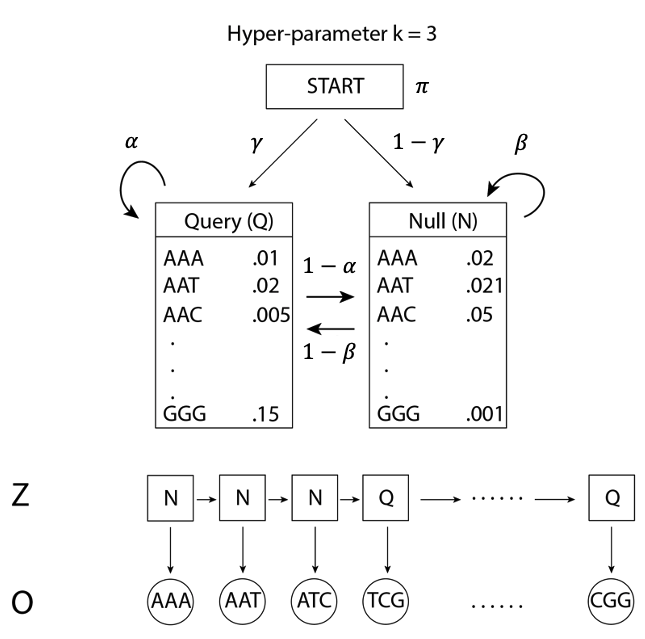
\includegraphics[width=\textwidth]{model.png}
\caption[Graphical model of \emph{hmmSEEKR}]{Graphical model of HMM SEEKR. The Query (``+") hidden state represents the functional domain to be identified in other lncRNA sequences and the Null (``-") hidden state represents the average $k$-mer frequencies of the transcriptome. The $\alpha$ and $\beta$ parameters represent the self-transition probabilities for the hidden state. }
\label{fig:hmmseekrmodel}
\end{figure}

\subsection{Parameter Estimation}
A hidden markov model is comprised of a stochastic transition matrix $A$, where each row vector $\psi_i$ corresponds to a categorical distribution representing hidden state $i$ probability of transitioning to state $j$. The emission matrix $E$, where each row corresponds to a categorical distribution of $k$-mer frequencies. Finally, there is the initialization matrix $\pi$ that describes the probability of starting at each hidden state at $t=1$.
\subsubsection{Emission Parameters}
We define the emission distribution for the query and null hidden states to be $k$-mer frequencies taken from a set of training sequences. For the query hidden state, we defined our training set to be \emph{XIST} repeats A,B,D, and E. For the null hidden state, we defined the set of training sequences to be the set of unspliced lncRNAs in the human transcriptome. 

The value of $k$ for each query was determined using a grid search based approach outlined in the Methods section below. Some of the \emph{XIST} repeats are quite short, for example \emph{XIST} repeat B is only $\approx 200$bp in length. Therefore, it is often the case that there are fewer nucleotides than there are parameters to estimate leading to zeros in the probability distribution. This is both unlikely, as many of the motifs for RBPs that bind \emph{XIST} have no non-zero probabilities, and also mathematically untractable, as we will need to work in log-space for probability calculations later.

To correct for this we employed pseudo-counts, specifically we use a $+1$ pseudo-count for all $k$-mers in the training set (\emph{i.e.} initialize the counts array to 1). The justification for this is relatively straightforward and rigorous. Given the transition matrix $A$, we know that each row vector within it is a categorical distribution $\phi$ comprised of all $k$-mer frequencies. Our hypothesis is that in spite of our limited training data, we believe that there is an underlying randomness, or probability distribution, to these $k$-mer frequencies, and we have not been able to sample enough sequence to account for that stochasticity. 

It can be shown that the \emph{maximum a posteriori}, or MAP, estimate for our $k$-mer frequency distribution is achieved by adding a pseudo-count of $1$ to each $k$-mer. This is achieved by placing a Dirichlet prior on our $k$-mer frequency distribution:

\begin{center}
    $\psi_i \sim Dir(\alpha_{AAA},\alpha_{AAT},\dots,\alpha_{GGG})$
    
    $x_i \sim Cat(\psi_{AAA},\psi_{AAT},\dots,\psi_{GGG})$
\end{center}

That is to say, the best estimate of the $k$-mer frequencies, given the data we have available and the uncertainty we have in it, is achieved by adding a count of $1$ to all $k$-mers. Intuitively this makes sense, as this addition has the largest impact when we have very little data to work with, and very little impact when we have substantial data as is the case for the null hidden state.

\subsubsection{Transition Parameters}

We are using the SEEKR algorithm to calculate which set of parameters for our HMM maximize the ‘distance’, or Kullback-Leibler diveregence, between a distribution of parsed and unparsed sequences.
The KL-Divergence is defined as \cite{Brookes1951FoundationsProbability}:
\begin{equation}
    D_{KL}(P||Q) = \sum_{x\in X}P(x)\log{\frac{P(x)}{Q(x}}
\end{equation}
Where $D_{KL}$ is the KL-Divergence between two probability distribtions P and Q. Here we will let P represent the SEEKR score distribution of the HMM parse hits to the query sequence, and Q represent the SEEKR score distribution of unparsed sequences to the query sequence, representing a ‘reference’. If P = Q then DKL = 0. D increases as the probability distributions become more dissimilar to each other. Important to note that $D_{KL}(P||Q) \neq D_{KL}(Q||P)$, so for consistenty $D_{KL}(P||Q)$ is always calculated.
Our goal is to find a set of parameters, $\alpha$ ($Q\rightarrow Q$), $\beta$ ($N\rightarrow N$), and k, that maximize the above expression
\begin{equation}
    \argmax_{\alpha,\beta,k}\sum_{x\in X}P(x|\alpha,\beta,k)\log{\frac{P(x|\alpha,\beta,k)}{Q(x|k)}}
\end{equation}


\begin{table}[h]
\centering
\begin{center}
 \begin{tabular}{|c | c| c | c |} 
 \hline
 Query & k & $\alpha$ & $\beta$ \\
 \hline\hline
 Repeat A & 4 & .9999 & .9999 \\ 
 \hline
 Repeat B & 4 & .9999 & .9999\\
 \hline
 Repeat D & 2 & .75 & .9999\\
 \hline
 Repeat E & 4 & .5 & .9999\\
 \hline
\end{tabular}
\end{center}
\caption{Best values of k, the $+\rightarrow +$ parameter $\alpha$, and $-\rightarrow -$ parameter $\beta$ as determined through a grid search based approach to identify sequences with the highest SEEKR correlation to the query.}
\label{tbl:transparams}
\end{table}

Being comprised of unparsed sequences, $Q(x)$ just depends on k.
In the real dataset, $P$ and $Q$ are histograms calculated from the data, and so the calculation of $D_{KL}$ compares the frequencies of SEEKR correlations in each bin for the two distributions. 

We found that $\beta$ must always be close to 1, whereas significant variance was found for the value of $\alpha$ amongst the different \emph{XIST} queries (Table \ref{tbl:transparams}). We also found that there was often significant overlap of hits between the varying sets of parameters (Fig \ref{fig:overlapparams})

\begin{figure}[h]
\centering
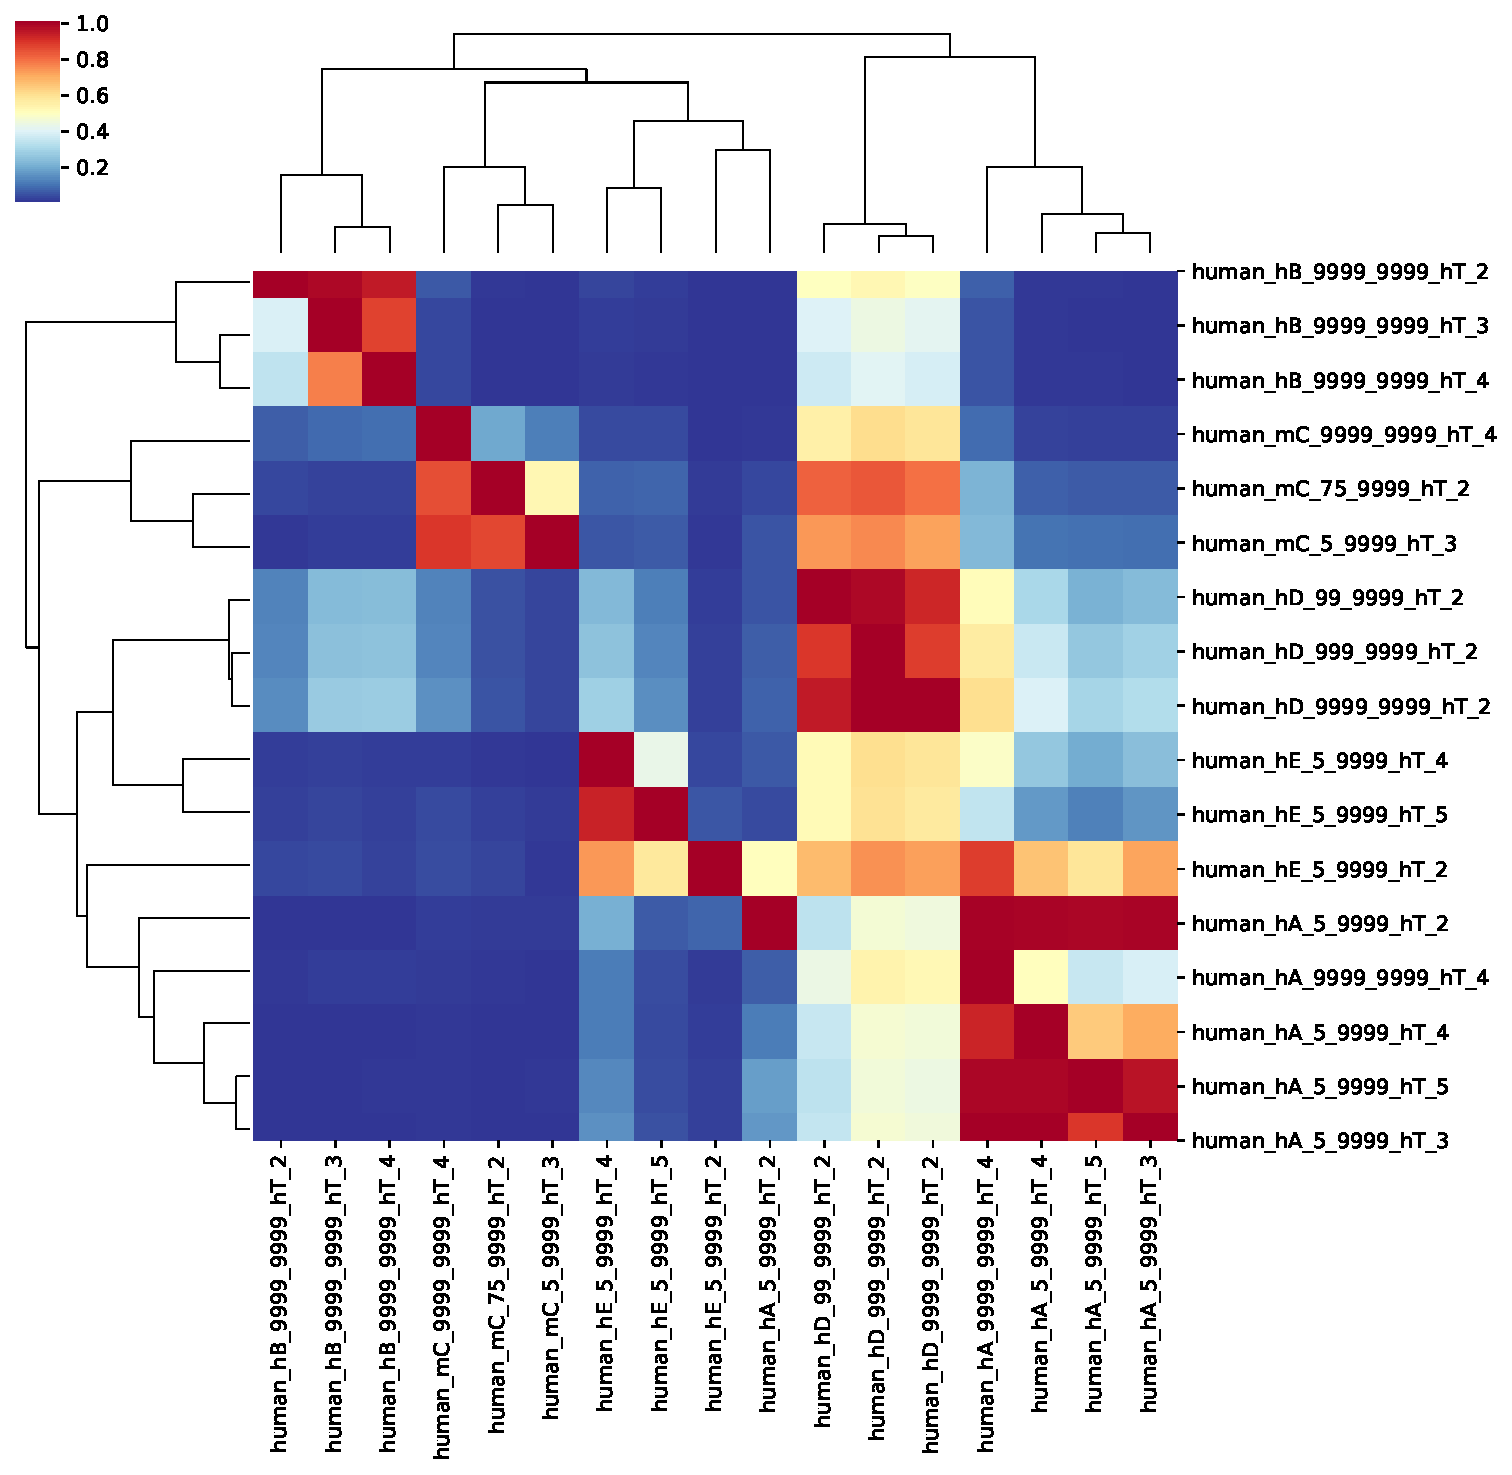
\includegraphics[width=\textwidth]{images/intersection.pdf}
\caption[Overlap of HMM hits with different parameterizations]{The fraction (colorbar) of shared HMM hits between different parameterizations and queries for \emph{hmmSEEKR}. Different HMM parameterization were clustered using complete linkage based on their degree of shared HMM hits.}
\label{fig:overlapparams}
\end{figure}

\subsection{Viterbi Parsing and Scoring}
The primary use for the HMM in \emph{hmmSEEKR} is identifying the most likely parse, $\phi_{max}$ for a given sequence or set of sequences, $X_i \in \{X_1,X_2,\dots,X_n\}$, where each $X_i$ is a sequence of $k$-mers. The regions that we define as ``hits" are all sub-sequences of contiguously query-labeled sequence, \emph{e.g.} for a sequence/parse pair such as:

$$(X_i=ATCGCCCG,\phi_{max}=-,-,+,+,+,+,+,+)$$

The ``hit" in this example as defined in \emph{hmmSEEKR} is the sub-sequence CGCCCG. There may be any number of hits within a sequence, but a hit is always composed of contiguous ``$+$" (query) labeled nucleotides.  The Viterbi path through each sequence was calculated as in algorithm \ref{alg:viterbi}, \ref{alg:backtrack}, and was implemented in corefunctions.py within the \emph{hmmSEEKR} package. This code can be called as in section 3.4.3 within the mSEEKR.py program.

Table \ref{tbl:hmmresults} illustrates the output of mSEEKR.py when scanning mouse \emph{Xist} using a human \emph{XIST} query. Here, an HMM was trained on human \emph{XIST} repeat A as the query hidden state, and the null hidden state was trained on the set of all unspliced lncRNAs in  mice (Methods 3.4.3,\cite{Derrien2012TheExpression}), and mouse \emph{Xist} was scanned for matches to the repeat A query. In the literature, repeat A is defined in mouse as spanning basepairs 292-713 \cite{Brockdorff10TheNucleus.}, and \emph{hmmSEEKR} called basepairs 201-748 as a hit to the repeat A query within mouse Xist (Table \ref{tbl:hmmresults}), yielding 100\% recovery of the original sequence. The score, kmerLLR as in table \ref{tbl:hmmresults}, is calculated as in Algorithm \ref{alg:LLR} and is the log-likelihood ratio of the hit. As the original definition for repeat A was formally defined by the presence of the tandem repeat \cite{Brockdorff10TheNucleus.,Brown10TheNucleus.}, and not based on functional motif enrichment or the presence of protein binding, it is significantly more challenging to accurately assess the false positive rate of the HMM.


\begin{table}[h]
\centering
\begin{tabular}{|l|l|l|l|l|l|}
\hline 
Rank&Start & End   & Length & kmerLLR & seqName                               \\
\hline 
0     & 201   & 748    & 547     & 285.225  & \textgreater{}xist \\
1     & 10295 & 11052  & 757     & 42.734   & \textgreater{}xist \\
2     & 1532  & 1576   & 44      & 30.685  & \textgreater{}xist \\
3     & 11326 & 11450  & 124     & 29.306   & \textgreater{}xist \\
4     & 17941 & 17946  & 5       & -0.968 & \textgreater{}xist\\
\hline 
\end{tabular}
\caption[\emph{mSEEKR.py output file}]{Output of \emph{mSEEKR.py}. Each hit from scanning \emph{XIST} with an HMM trained on the A-repeat of mouse \emph{Xist} is shown and sorted by the \emph{hmmSEEKR} score, ``kmerLLR". }
\label{tbl:hmmresults}
\end{table}

As there are no pre-existing annotations for these $k$-mer based sequence features within lncRNAs, it is difficult to define what constitutes a true positive and a true negative. To help elucidate what sequence features within \emph{XIST} and other lncRNAs are functional, we turned to protein binding data for proteins that are known to bind \emph{XIST} and have been shown to be crucial for its function.

\subsection{Xist Associated RBPs}
A crucial feature of the \emph{XIST} transcript are the 4 core repeats that bind unique subsets of RNA binding proteins \cite{Sunwoo2017RepeatCIZ1,Zhao2008PolycombChromosome,Pintacuda2017HnRNPKSilencing,Wang2017TargetingGuanines,Hoki2009AMouse}. Several RBPs have been shown to be crucial for the function of \emph{XIST}, including HNRNPK, RBM15, and several others \cite{Sunwoo2017RepeatCIZ1,Zhao2008PolycombChromosome,Pintacuda2017HnRNPKSilencing,Wang2017TargetingGuanines,Hoki2009AMouse,Chu2015SystematicProteins}. The tandem repeats have been defined based off their repetitiveness, but Figure \ref{fig:shufD} demonstrates that a non-repetitive sequence can have the same motif content as a repetitive one. Indeed, examination of ENCODE eCLIP data for HNRNPK reveals significant eCLIP binding adjacent to and extending beyond the formally defined B- and D-repeats of \emph{XIST}. Therefore, we hypothesized that the functional elements of lncRNA such as \emph{XIST} are not defined by repetitiveness but rather by enrichment of protein binding motifs \cite{Kirk2018FunctionalContent,Sprague2019NonlinearDomains,Dominguez2018SequenceProteins,Ray2013ARegulation,Wang2017TargetingGuanines}. To further test \emph{hmmSEEKR}, we sought to identify the proteins most associated with the A,B,D,E-repeats of \emph{XIST} so that we could validate the predictive power of our model against existing protein binding data.
\begin{figure}[h!]
\centering
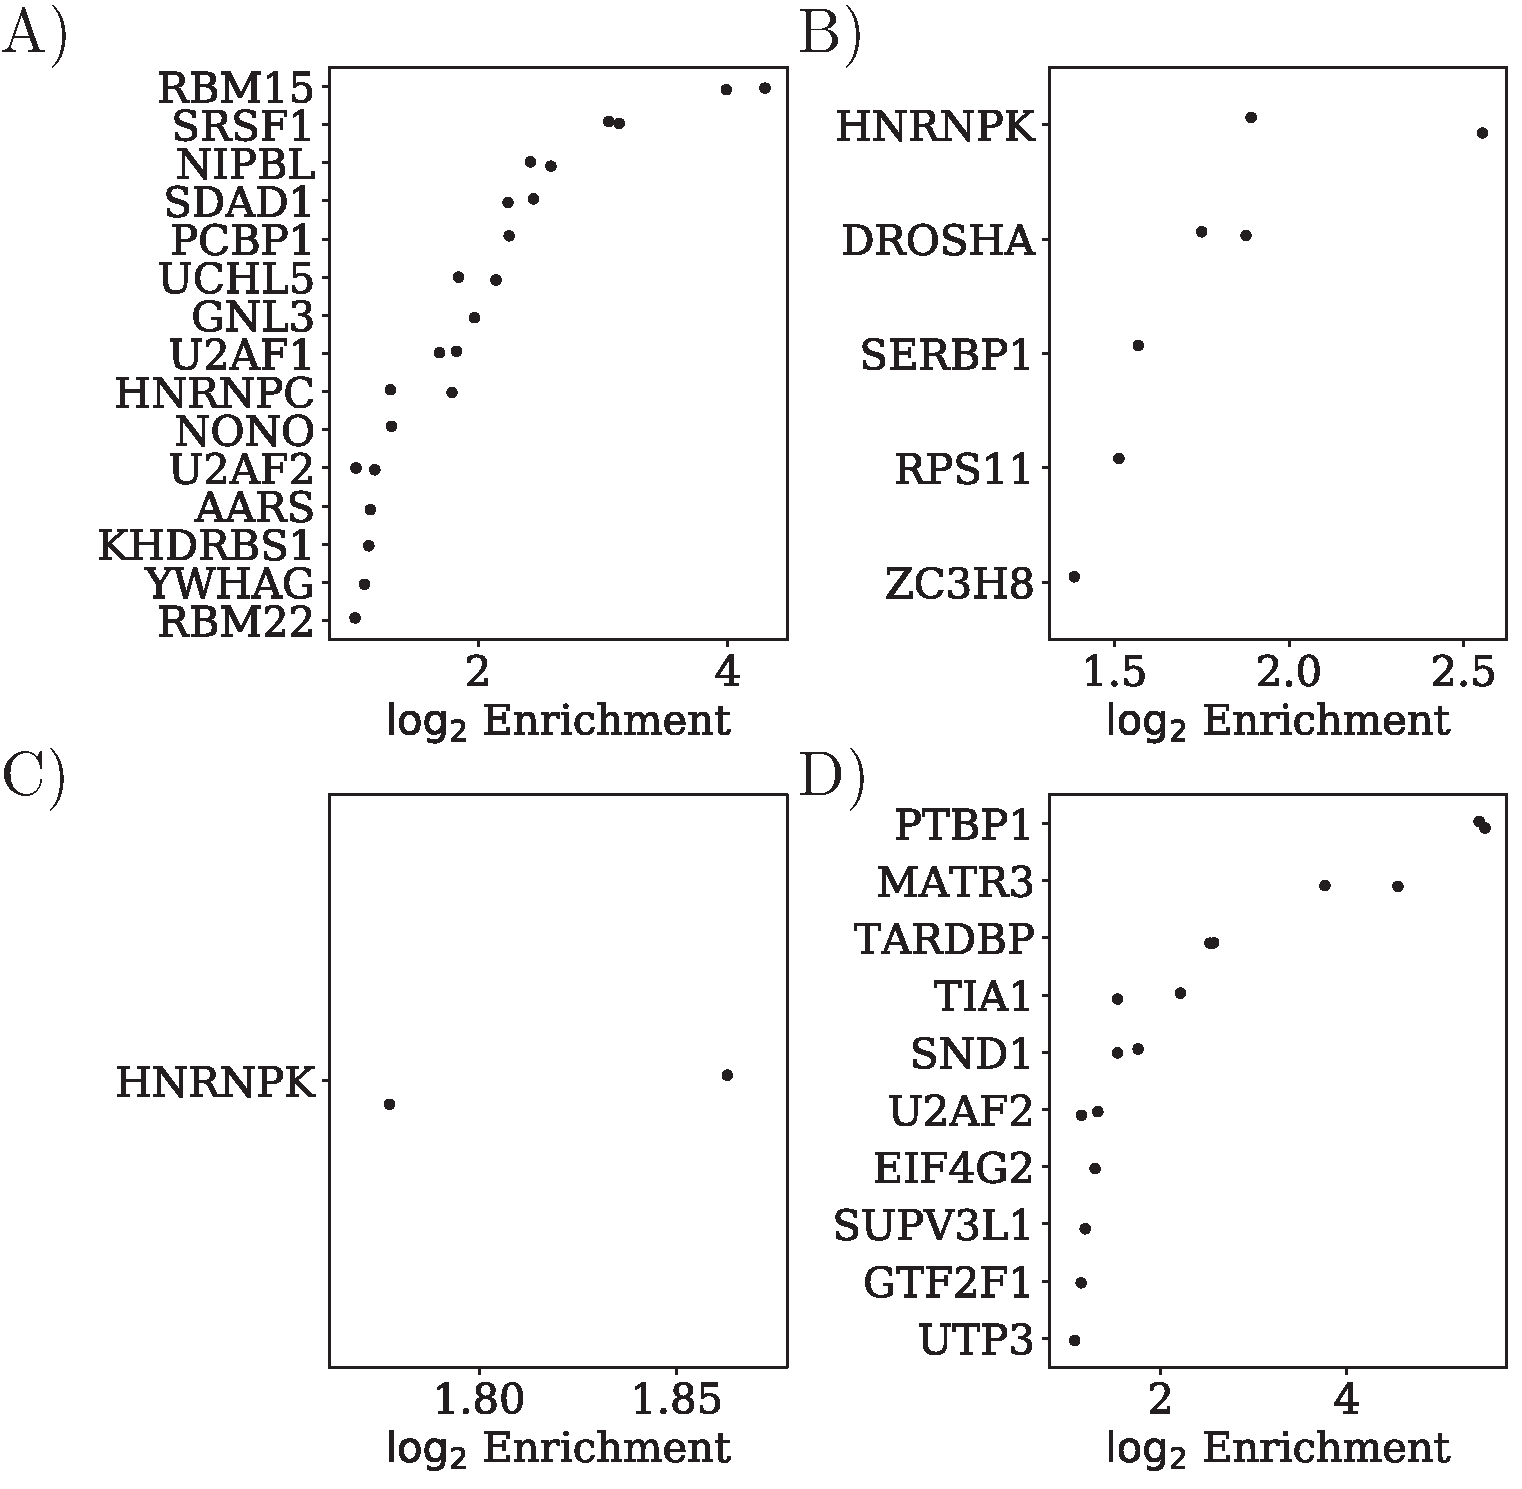
\includegraphics[width=\textwidth]{images/sigproteins.pdf}
\caption[\emph{XIST} tandem repeat enriched proteins]{Proteins selectively enriched within tandem repeats of \emph{XIST}. A) $\log_2$ ratio of read density for Repeat A compared to the remainder of \emph{XIST}. Individual points represent biological replicates. B) $\log_2$ ratio of read density for Repeat B compared to the remainder of \emph{XIST} is shown. Individual points represent biological replicates. C) $\log_2$ ratio of read density for Repeat D compared to the remainder of \emph{XIST}. Individual points represent biological replicates. D) $\log_2$ ratio of read density for Repeat E compared to the remainder of \emph{XIST}. Individual points represent biological replicates.}
\label{fig:xistproteins}
\end{figure}

We found that each repeat within \emph{XIST} contained at least one protein that was at least 2x more enriched in within the repeat than the remainder of the \emph{XIST} transcript (Figure \ref{fig:xistproteins}A). RBM15 and SRSF1 were found to be the most specific proteins to repeat A. Prior work has shown that RBM15 is required for full \emph{XIST} silencing functionality, and that RBM15 recruits the m6A complex to the 5' region of \emph{XIST}. SRSF1 has previously been shown to bind the A-repeat of \emph{XIST} but its function within the sequence is currently unknown.


Both the B-repeat and D-repeat were found to be significantly enriched for HNRNPK over the rest of the transcript (Figure \ref{fig:xistproteins}B-C). HNRNPK is required for recruitment of PRC1 to the \emph{XIST} transcripts. Deletion of the B-repeat region has previously been shown to be sufficient to abrogate \emph{XIST} dependent PRC recruitment, as well as \emph{XIST} mediated silencing. Our analysis showed that DROSHA is also enriched within the B-repeat of \emph{XIST}, however no previous studies have identified DROSHA as a direct interactor with \emph{XIST} and so the function of this interaction is unknown.

\begin{table}[h]
\centering
\begin{tabular}{|l|l|}
\hline 
\emph{Xist} Repeat&eCLIP Data                      \\
\hline 
    A&RBM15,SRSF1    \\
      B & HNRNPK\\
      D  & HNRNPK\\
      E & TIA1,MATR3,PTBP1\\
\hline 
\end{tabular}
\caption{Most enriched RBPs for each tandem repeat domain in \emph{XIST}. }
\label{tbl:eclipscan}
\end{table}

The E-repeat of \emph{XIST} was highly enriched for several proteins. The E-repeat itself is composed primarily of T-rich sequence, and therefore the proteins we observe often contain similar motifs (cisBP). PTBP1, MATR3, TARDBP, and TIA1 were all found to be the most enriched within the E-repeat. PTBP1 has previously been shown to be required for proper \emph{XIST} expression and splicing during development. TARDBP depletion is also associated with increased expression of mis-spliced \emph{XIST} transcripts. A recent study found that MATR3 and PTBP1 form a condensate mediated by the \emph{XIST} E-repeat and this condensate is required for \emph{XIST} localization to the Xi. 

\subsection{Detection of Rsx Domains}
Our \emph{Rsx} study in Chapter 2 relied on the existence of tandem repeats within the \emph{Rsx} transcript to perform the domain based SEEKR analysis. On a whole transcript level, \emph{XIST} and \emph{Rsx} were slightly anti-correlated despite their shared function. The relationship between the two sequences didn't become apparent until we parsed out the tandem repeats within \emph{Rsx} and performed pairwise comparisons between each \emph{XIST} tandem repeat. 

We hypothesized that we could use \emph{hmmSEEKR} to identify regions of non-linear sequence similarity between \emph{XIST} and \emph{Rsx} without \emph{a priori} identification of tandem repeats. To do this, we trained 4 separate HMMs on the A,B,D, and E-repeats of \emph{XIST} at $k=2,3,4,5,6$ and all pairwise combinations of $\alpha,\beta = .5,.75,.9,.99,.999,.9999$. The results outlined in Figure \ref{fig:koalarsxhmm} and Table \ref{tbl:rsxresults} are using the set of parameters that yielded the best F1 score (Methods 3.4.X). 


\begin{figure}[h!]
\centering
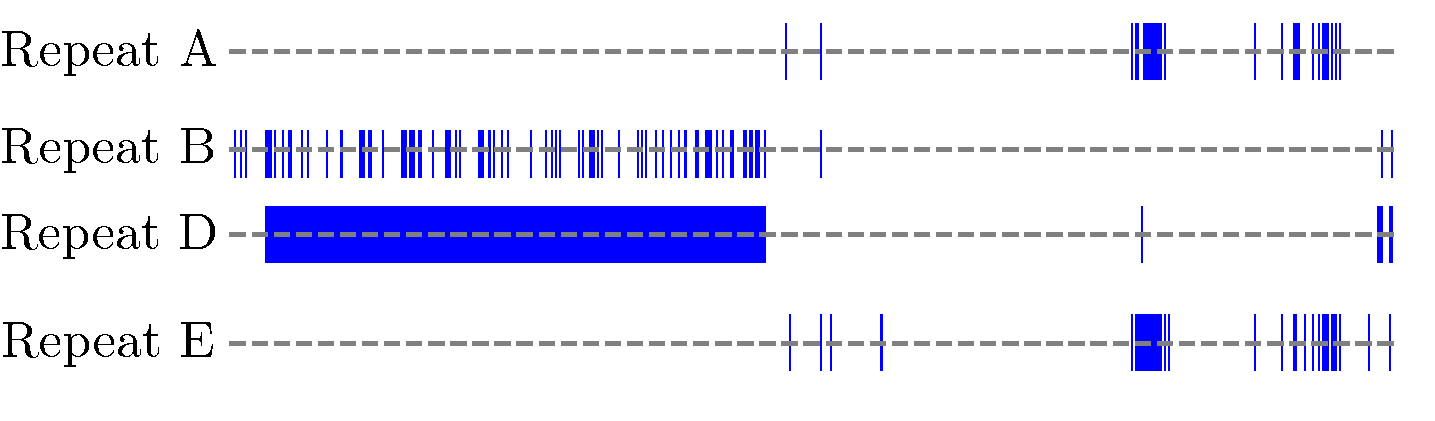
\includegraphics[width=\textwidth]{images/koalarsx.pdf}
\caption[HMM analysis of \emph{Rsx}]{\emph{hmmSEEKR} hits within \emph{Rsx} for an HMM trained on each \emph{XIST} repeat. Blue regions represent hits to the query, whereas dashed grey lines represent null sequence.}
\label{fig:koalarsxhmm}
\end{figure}

We found that the HMM trained on the \emph{XIST} D-repeat captured the entire tandem repeat from transcript coordinates 1,000-14,000 (Figure \ref{fig:koalarsxhmm}, Table \ref{tbl:rsxresults}). Likewise, the HMM trained on the \emph{XIST} B-repeat captured a significant portion of \emph{Rsx} repeat 1, and these regions were significantly more C-rich than the remainder of \emph{Rsx} repeat 1 (show data). Additional C-rich sequence were also identified at the 5' and 3' regions of \emph{Rsx} (Figure \ref{fig:koalarsxhmm}). The HMMs trained on the A-repeat and E-repeat both significantly aligned with \emph{Rsx} repeat 4, with 100\% precision and 25.45\% recall. In our original analysis, we mapped A,E-repeats to repeats 2,3, and 4 in \emph{Rsx}, however repeats 2 and 3 had relatively marginal correlation to the A,E-repeats, whereas the A,E$\rightarrow$4 relationship was the strongest of all comparisons in the original \emph{Rsx} analysis (Sprague et al.).

\begin{table}[h!]
\centering
\begin{tabular}{|l|l|l|l|l|l|}
\hline 
\emph{Rsx} Repeat Name& Start & End   & Xist Association   & Precision& Recall                      \\
\hline 
    1&  1000   & 14000    & B,D     & 98.42\% & 100\% \\
      2&17500 & 21000  & A,E     & 100\%   & 1.32\% \\
      3&21500  & 22500   & A,E      & 0\% & 0\%  \\
      4&23000 & 27500  & A,E     & 100\%   & 25.45\% \\
\hline 
\end{tabular}
\caption{Precision and recall for each HMM using the tandem repeat definitions from \cite{Sprague2019NonlinearDomains}. Precision is defined as the number of correct nucleotides relative to the number of incorrect nucleotides, whereas recall is the fraction of the total domain retrieved by the HMM.}
\label{tbl:rsxresults}
\end{table}


\subsection{Sequence based prediction of RBP binding in Kcnq1ot1}

\begin{figure}[h!]
\centering
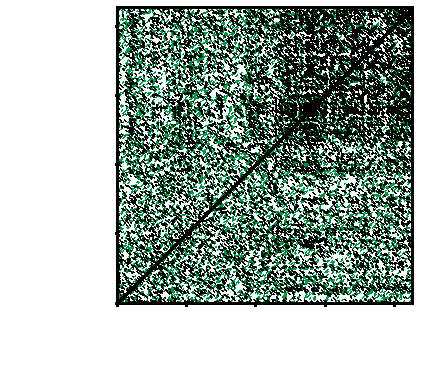
\includegraphics[width=.4\textwidth]{images/kcnd.pdf}
\caption[\emph{KCNQ1OT1} dot plot alignment]{Dot plot alignment of human \emph{KCNQ1OT1} against itself using flexidot software \cite{Flexidot}. The window parameter is 20bp and the threshold is 40\%. Black regions correspond to windows that succesfully aligned against each other. }
\label{fig:kcndot}
\end{figure}

There is at least one lncRNA in the human transcriptome that is known to silence gene expression in \emph{cis} through a PRC-mediated mechanism similar to \emph{XIST}, \emph{KCNQ1OT1}. The mouse \emph{Kcnq1ot1} has been shown to silence megabase scale regions of chromosome 7 and human \emph{KCNQ1OT1} silences a large region of chromosome 11. Unlike \emph{XIST}, the sequence of \emph{KCNQ1OT1} is not predominantly comprised of tandem repeat domains (Figure \ref{fig:kcndot}), barring a region in the 3' region of the sequence. Furthermore, eCLIP data for RBPs known to be essential for \emph{XIST}'s function show that the predominantly bind in the 5' half of \emph{KCNQ1OT1}'s sequence (Figure \ref{fig:kcnproteins}). Therefore, we sought to use the \emph{hmmSEEKR} package to identify functional sub-sequences within \emph{KCNQ1OT1} that are similar in $k$-mer content to \emph{XIST} A-,B-,D-, and E-repeats. 


\begin{figure}[h!]
\centering
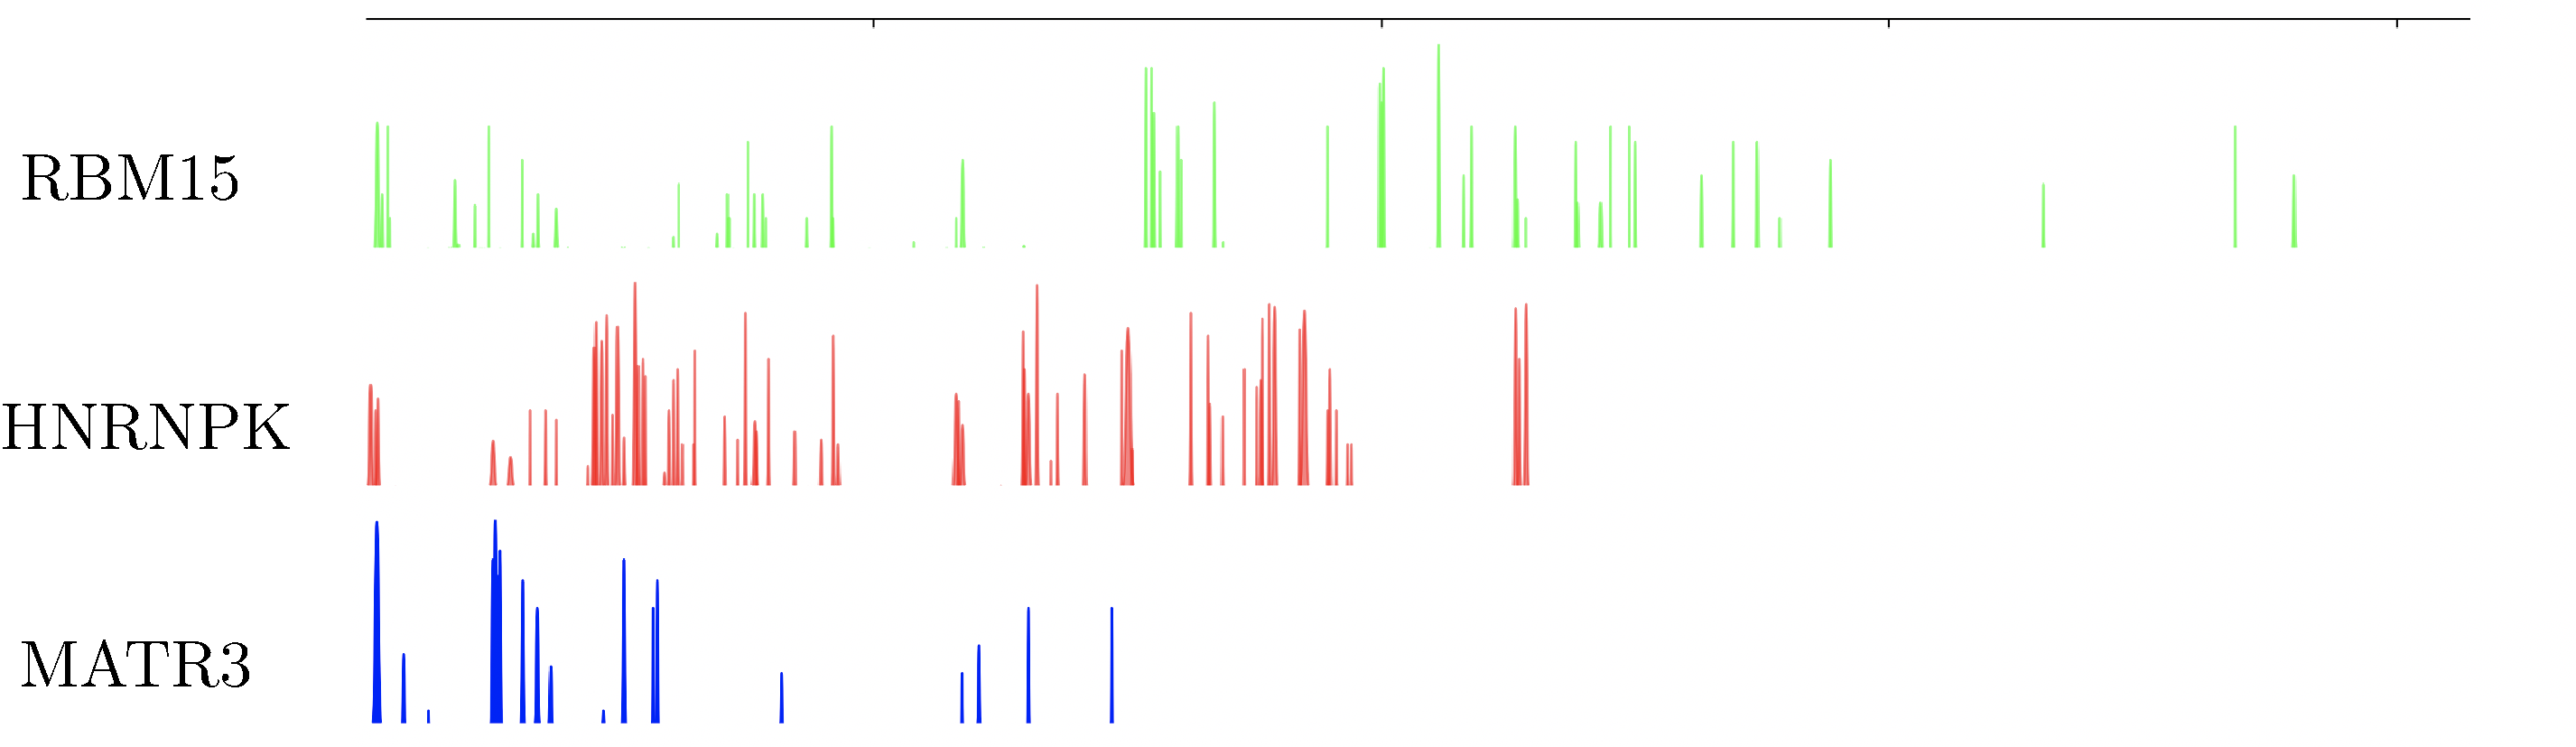
\includegraphics[width=\textwidth]{images/kcnproteins.pdf}
\caption[\emph{KCNQ1OT1} RBM15, HNRNPK, and MATR3 eCLIP tracks]{Browser tracks for RBM15 (top), HNRNPK (middle), and MATR3 (bottom) within the \emph{KCNQ1OT1} locus. Data shown are the eCLIP narrowPeak files for each protein.}
\label{fig:kcnproteins}
\end{figure}

\emph{KCNQ1OT1} contained regions of similarity to each of the \emph{XIST} HMMs that we trained (Figure \ref{fig:kcntracks} A-D). We found that the 5' region of \emph{KCNQ1OT1}'s sequence in particular containins regions of similarity to A-,B-,D-, and E-repeats of \emph{XIST} (Figure \ref{fig:kcntracks} A-D) -- suggesting that this region of \emph{KCNQ1OT1} is multipurpose binder of RBPs. Indeed, eCLIP data for RBM15 and SRSF1 (Figure \ref{fig:kcntracks} A), HNRNPK (Figure \ref{fig:kcntracks} B-C), and MATR3 and PTBP1 (Figure \ref{fig:kcntracks} D) reveal elevated read density for all these proteins at the 5' region of \emph{KCNQ1OT1}'s sequence. Additionally, a large portion of the inner region of \emph{KCNQ1OT1}'s sequence was identified by \emph{hmmSEEKR} to have similarity to the B- and D- repeats of \emph{Xist}. (Figure \ref{fig:kcntracks} B-C). Similar to actual B- and D-repeats of \emph{XIST}, these regions within \emph{KCNQ1OT1} correspond to elevated HNRNPK read density (Figure \ref{fig:kcntracks} B,C). 
\begin{figure}[h!]
\centering
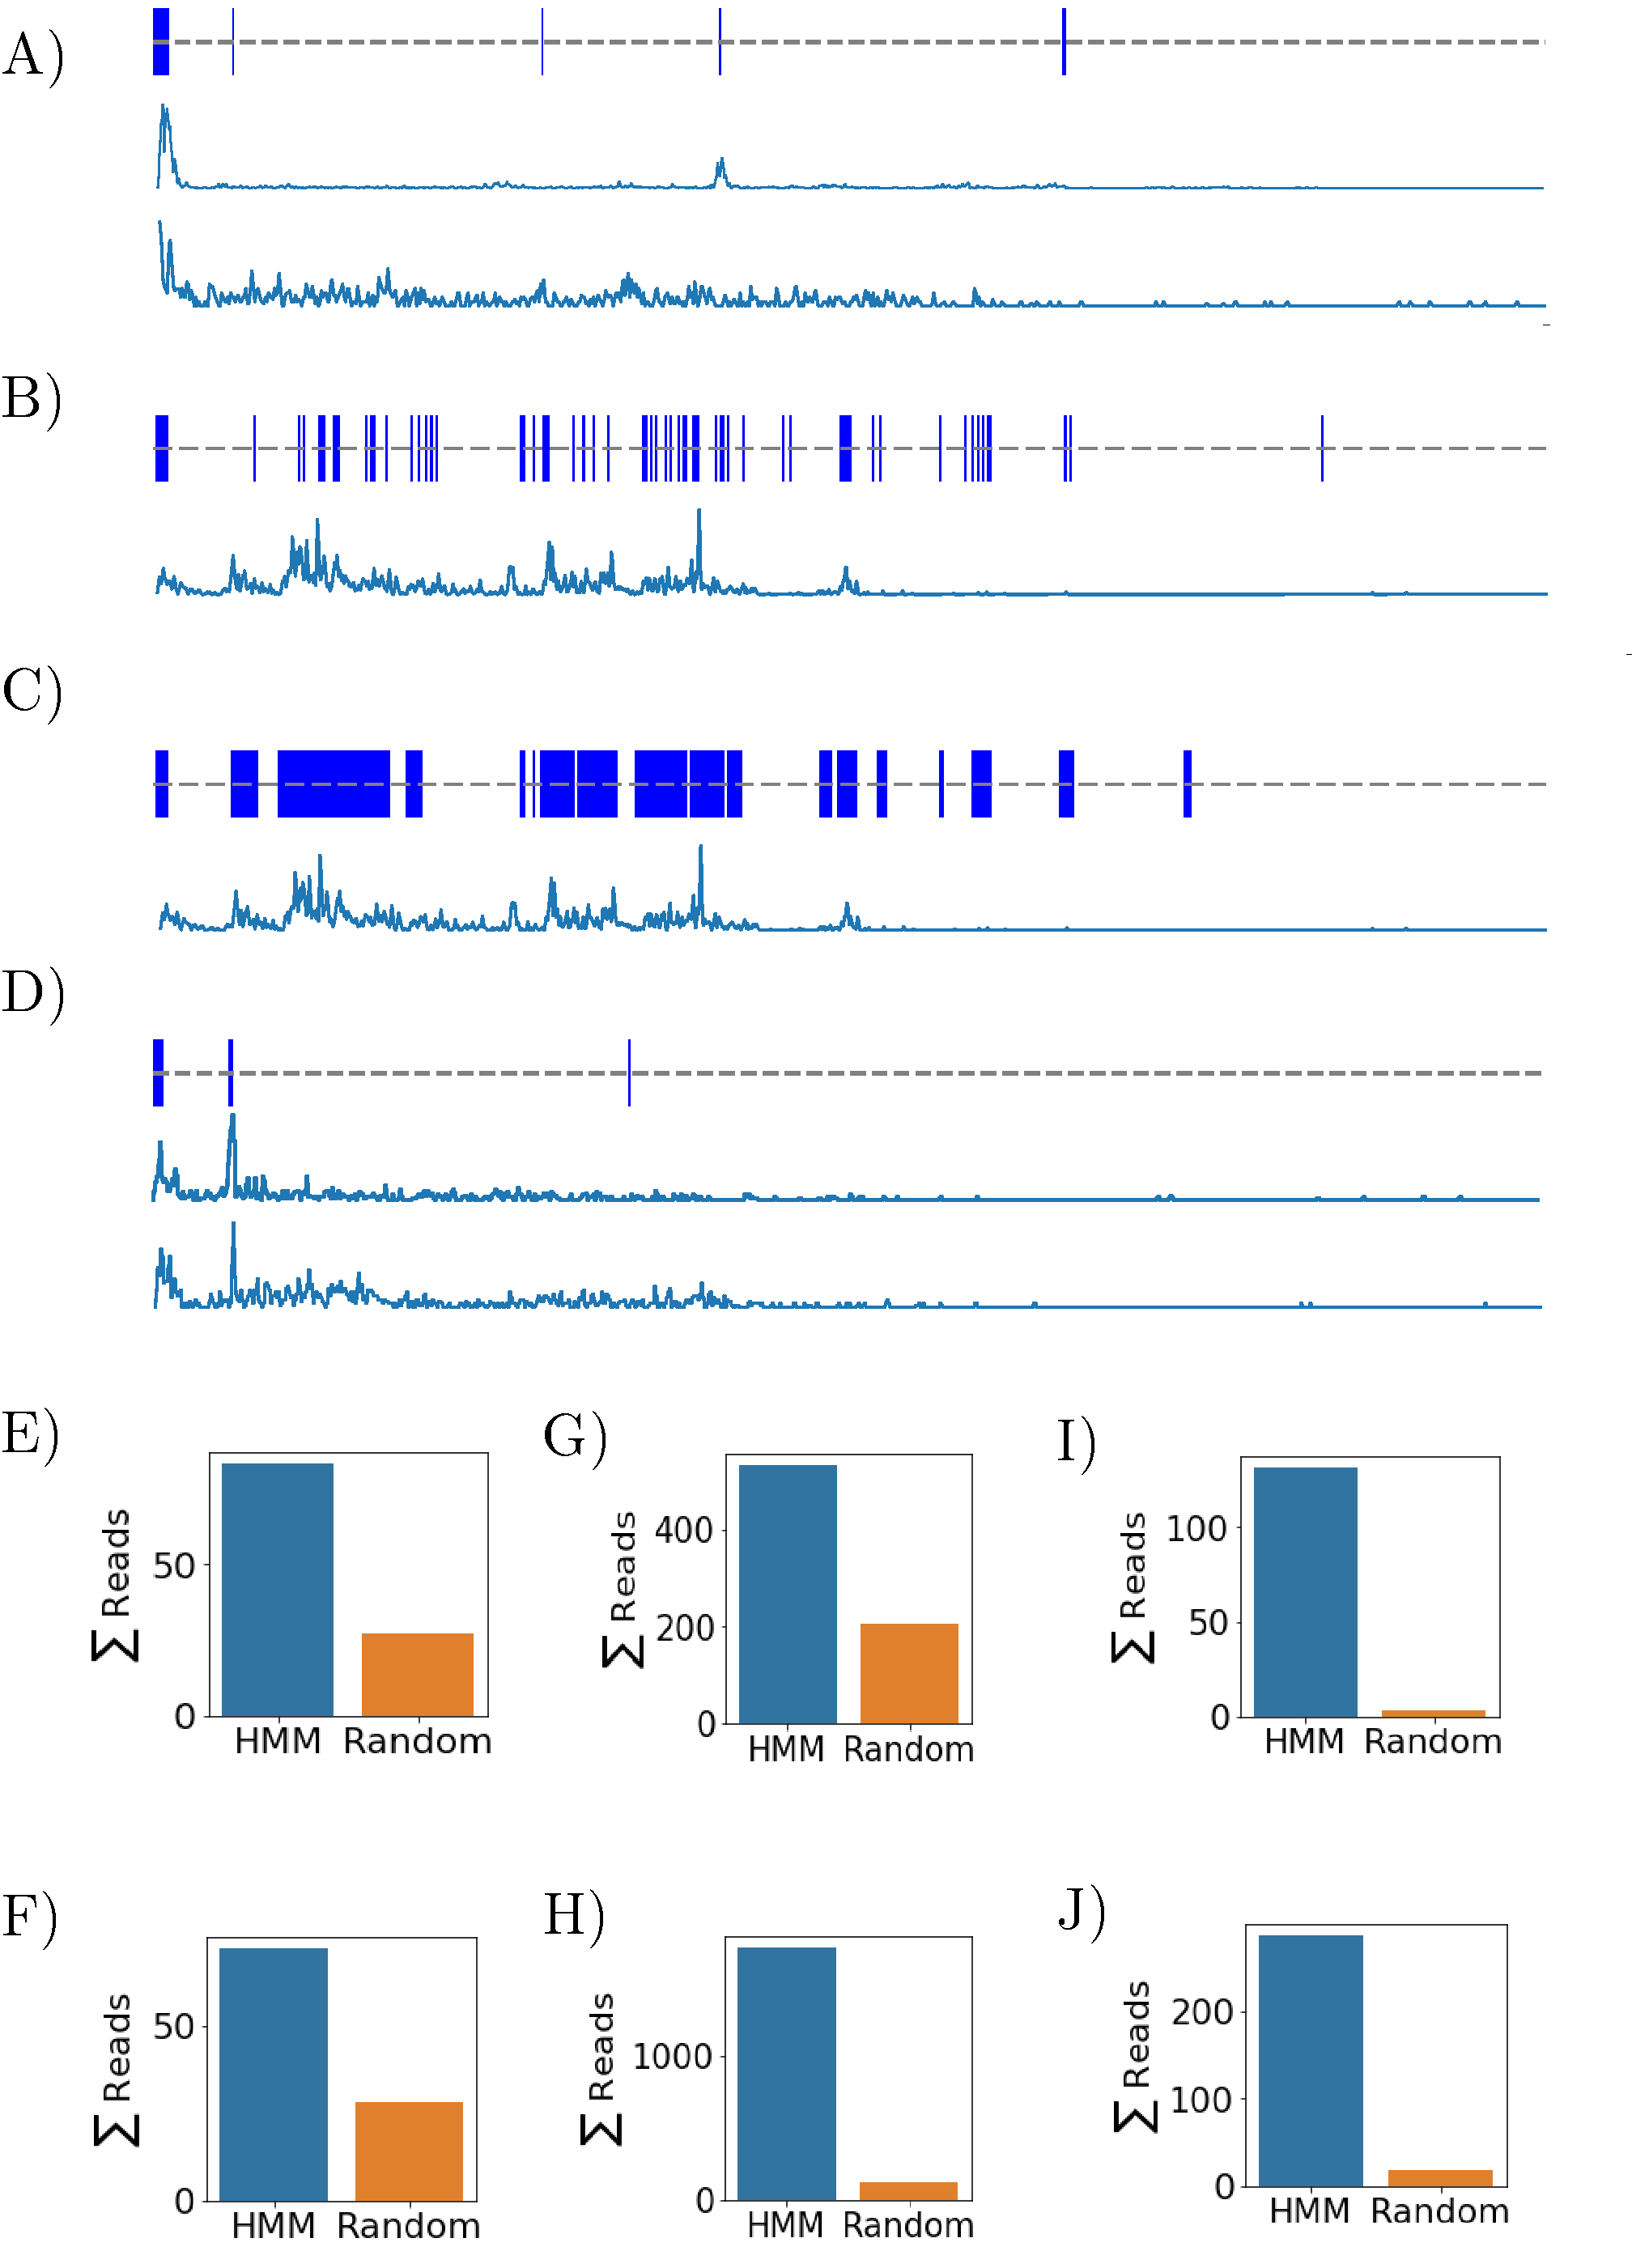
\includegraphics[width=.92\textwidth]{images/kcneclip.pdf}
\caption[Analysis of HMM and eCLIP data in \emph{KCNQ1OT1}]{\emph{hmmSEEKR} predicts \emph{XIST} associated protein binding in \emph{KCNQ1OT1}. A) HMM viterbi parse showing hits to the A-repeat in \emph{KCNQ1OT1} (blue), RBM15 eCLIP read density (middle plot), and SRSF1 eCLIP read density (bottom plot). B) HMM viterbi parse showing hits to the B-repeat (top, blue regions), and HNRNPK eCLIP read density (bottom). C) HMM viterbi parse in \emph{KCNQ1OT1} for the D-repeat (top, blue regions) and HNRNPK eCLIP read density (bottom). D) HMM viterbi parse for E-repeat in \emph{KCNQ1OT1} (top, blue regions) and eCLIP read density for MATR3 (middle) and PTBP1 (bottom). E-J) Total eCLIP reads assigned to the HMM or randomized parses for RBM15, SRSF1, HNRNPK (B-repeat), HNRNPK (D-repeat), MATR3, and PTBP1 respectively. }
\label{fig:kcntracks}
\end{figure}

We then sought to compare the read density for each protein in Table \ref{tbl:eclipscan} found within our \emph{hmmSEEKR} prediction for the associated \emph{XIST} query against a randomized shuffling of the hits found within \emph{KCNQ1OT1} (Method 3.4.6 randomization). We found that the A-repeat HMM significantly outperformed randomized shuffles for both RBM15 (Figure \ref{fig:kcntracks} E; $p< 10^{-8}$, chi-square test) and SRSF1 (Figure \ref{fig:kcntracks} F; $p< 10^{-5}$, chi-square test). HNRNPK was also significantly better predicted by the HMMs trained on the B- and D-repeats of \emph{XIST} (Figure \ref{fig:kcntracks} G,H;$p<10^{-33}$ B-repeat, $p<10^{-51}$ D-repeat, chi-square test). Finally, the E-repeat trained HMM significantly outperformed a shuffled parse for both MATR3 (Figure \ref{fig:kcntracks} I, $p<10^{-28}$,chi-square test) and PTBP1 (Figure \ref{fig:kcntracks} J; $p<10^{-43}$,chi-square test). 

\clearpage


%%%%%%%%%%%%%%%%%%%%%
%%%%%%%%%%%%%%%%%%%%%

\subsection{Transcriptome-wide RBP Prediction}
Many of the proteins that bind to \emph{XIST} and \emph{KCNQ1OT1} bind throughout the transcriptome \cite{VanNostrand2016RobusteCLIP}. Furthermore, \emph{XIST} clusters with thousands of transcripts in the human genome based on $k$-mer content \cite{Kirk2018FunctionalContent}. Therefore, we hypothesized that \emph{XIST}-like sub-sequences may be found throughout the transcriptome, both in lncRNAs as well as in pre-mRNAs. To test this hypothesis, we trained 4 HMMs on the A-,B-,D-, and E-repeats of human \emph{XIST} as in section 3.2.6 and used \emph{hmmSEEKR} to scan the set of all unspliced coding and non-coding transcripts in the human genome. We compared the results of our HMM against ENCODE eCLIP data for proteins that we have shown are enriched within each \emph{XIST} repeat (Table \ref{tbl:eclipscan}). 

The \emph{hmmSEEKR} HMMs significantly out-performed randomized HMM parses for each of the proteins we tested. The A-repeat trained HMM successfully captured significantly more reads for RBM15 (Figure \ref{fig:transcriptome} A left; $p\ll 10^{-100}$, chi-squared test) and SRSF1 (Figure \ref{fig:transcriptome} B left panels; $p\ll 10^{-100}$, chi-squared test) than did the randomized hits. Furthermore, true HMM hits throughout the transcriptome had significantly more reads per hit than the shuffled parses for RBM15 eCLIP data (Figure \ref{fig:transcriptome} A right panel; $p\ll10^{-100}$, student's t-test) and SRSF1 (Figure \ref{fig:transcriptome} B right panel; $p\ll10^{-100}$,student's t-test).

\begin{figure}[h!]
\centering
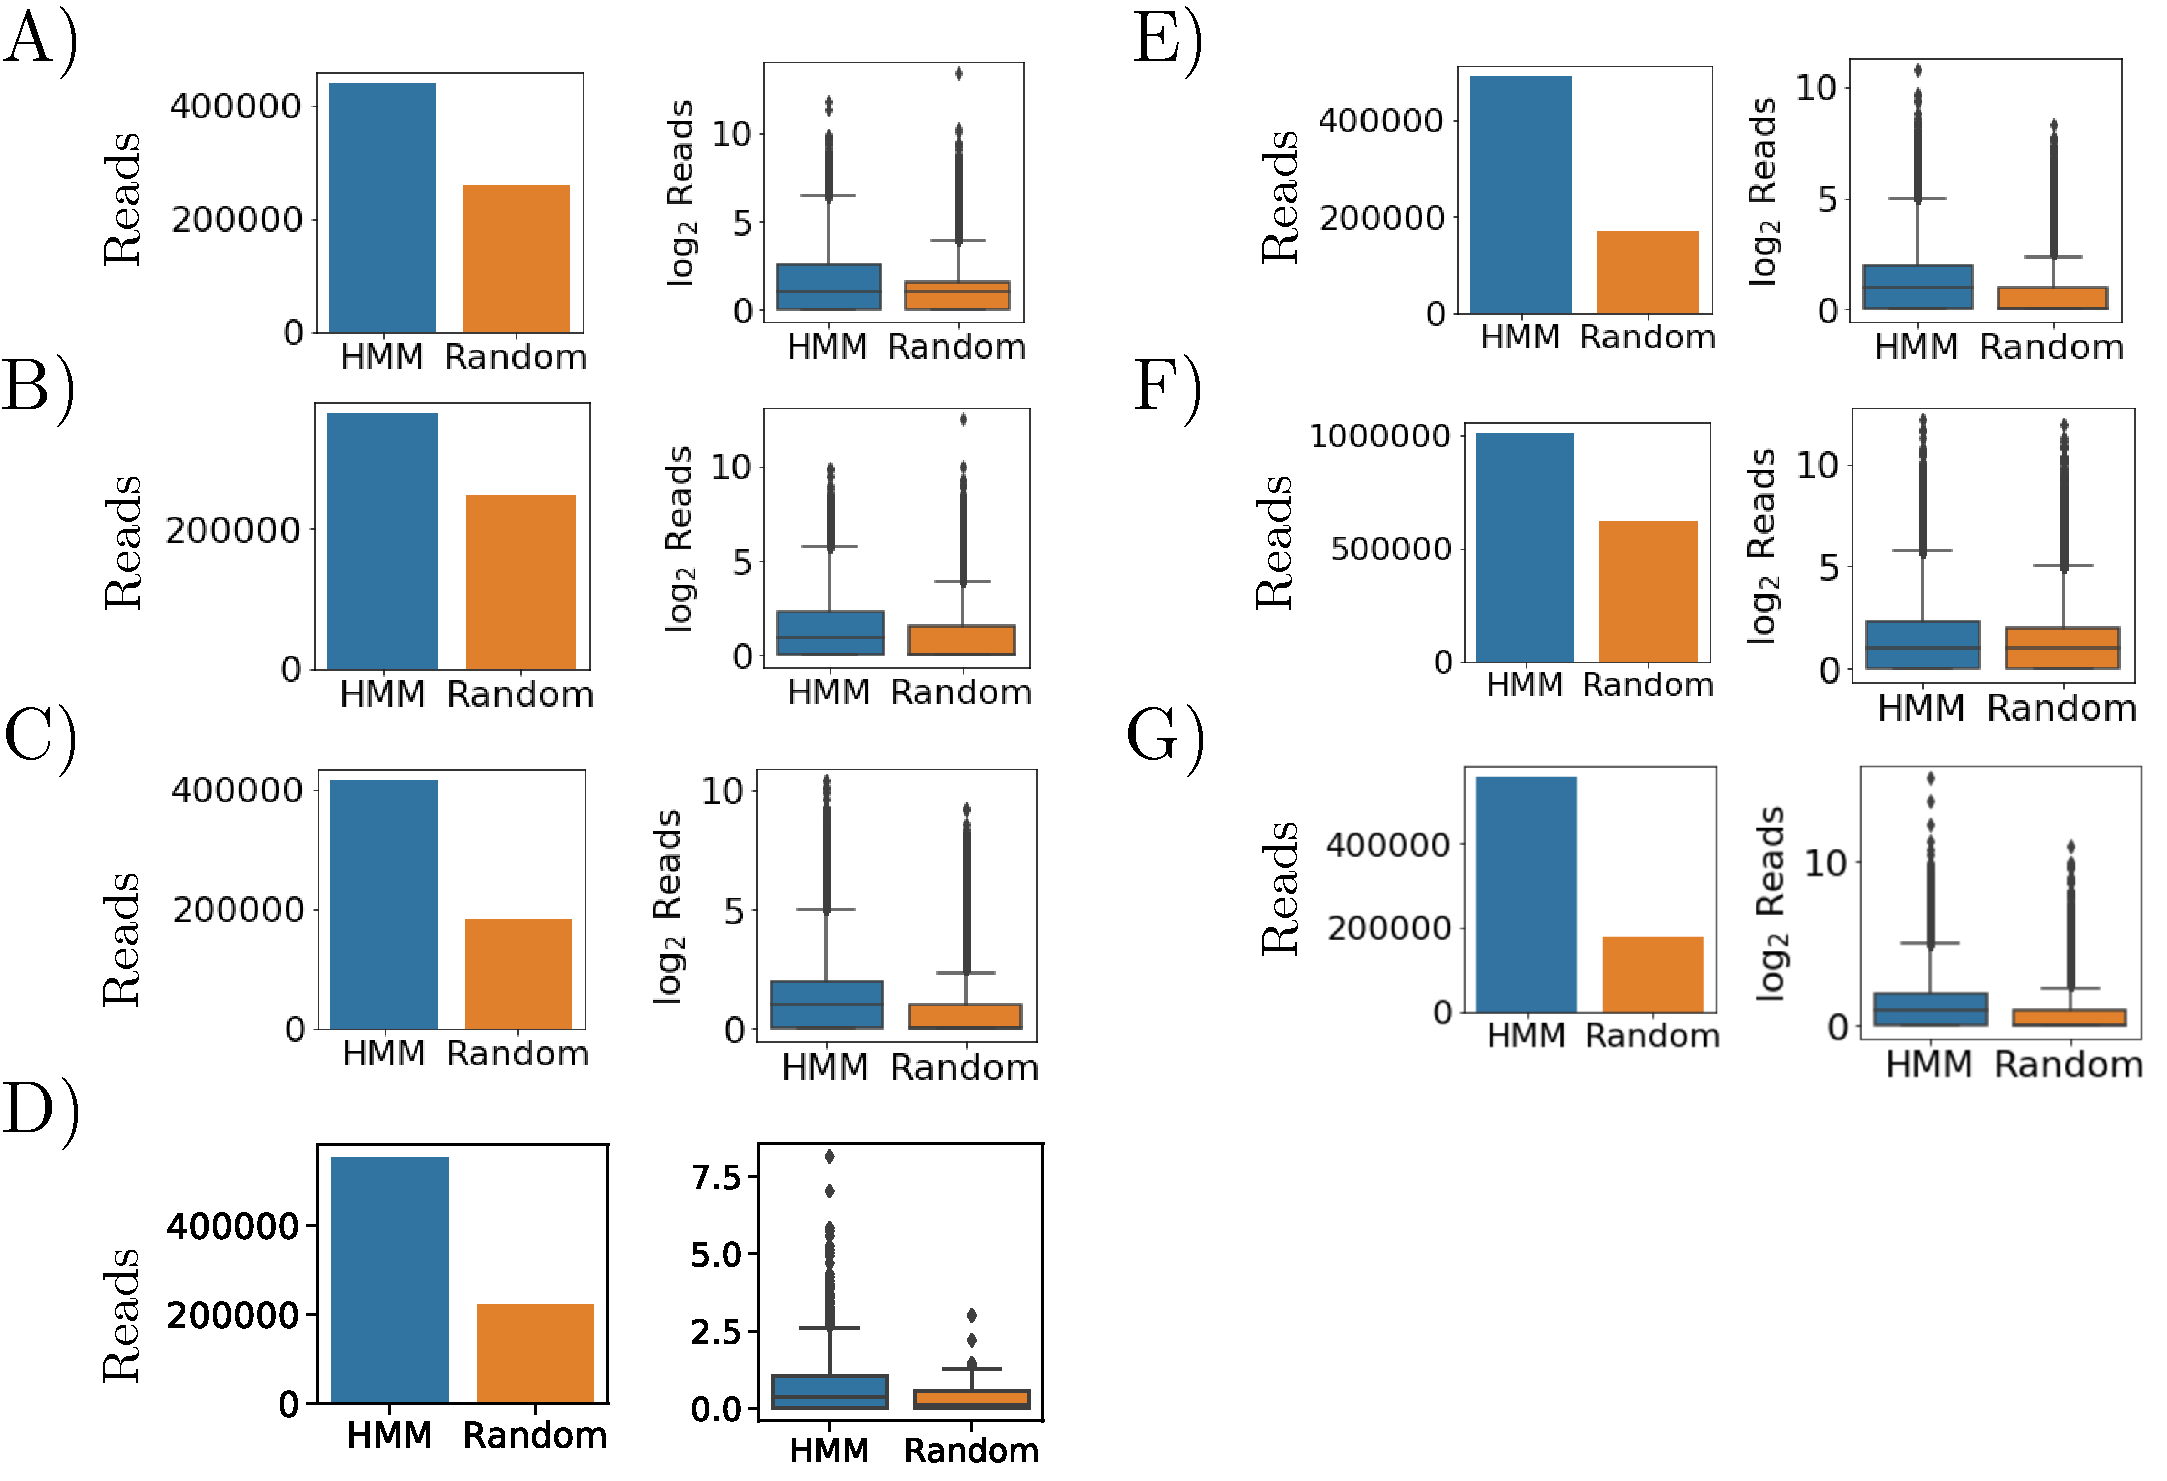
\includegraphics[width=.95\textwidth]{images/transcriptomescan.pdf}
\caption[Transcriptome-wide prediction of RBP binding regions]{\emph{hmmSEEKR} models trained \emph{XIST} tandem repeats predict RBP binding regions throughout the transcriptome. A-G) Total number of eCLIP reads assigned to HMM Viterbi parse hits compared to randomized shuffling of hits within each transcript (left plot), and the number of reads per hit for the true HMM hits compared to the shuffled parses (right plots), for RBM15 (A), SRSF1 (B), HNRNPK B-repeat (C), HNRNPK D-repeat (D), MATR3 (E), TIA1 (F), PTBP1 (G).}
\label{fig:transcriptome}
\end{figure}

The B-repeat trained model had significantly more reads assigned from HNRNPK eCLIP data (Figure \ref{fig:transcriptome} C left-panel, $p\ll10^{-100}$, chi-squared test), and significantly more reads per hit than the randomized parses (Figure \ref{fig:transcriptome} C right-panel, $p\ll10^{-100}$,student's t-test). A similar pattern emerged with the D-repeat HMM, which captured more reads than the B-repeat HMM (Figure \ref{fig:transcriptome} C-D left-panels), and overlapped significantly more reads than randomized parses (Figure \ref{fig:transcriptome} D left-panel, $p\ll10^{-100}$,chi-square test) as well as more reads per hit than the randomized parses (Figure \ref{fig:transcriptome} D right-panel, $p\ll10^{-100}$,student's t-test). 

Finally, the E-repeat trained HMM also successfully predicted associated protein binding better than randomized parses (Figure \ref{fig:transcriptome} E-G). MATR3 had significantly more reads assigned by the true HMM (Figure \ref{fig:transcriptome} E left-panel, $p\ll 10^{-100}$,chi-square test) and more reads per hit than random (Figure \ref{fig:transcriptome} E right-panel, $p\ll 10^{-100}$, student's t-test). Intriguingly, the HMM assigned significantly more reads from TIA eCLIP (Figure \ref{fig:transcriptome} F left-panel, $p\ll 10^{-100}$, chi-squared test) but there was no significant difference in the number of reads per hit for the true HMM parses and the randomized parses (Figure \ref{fig:transcriptome} F right-panel, \emph{n.s.}, student's t-test). PTBP1 displayed the highest ratio of assigned reads between the true HMM and randomized parses over all comparisons (Figure \ref{fig:transcriptome} A-G left-panels) and assigned significantly more eCLIP reads than the randomized parses (Figure \ref{fig:transcriptome} G left-panel, $p\ll10^{-100}$, chi-squared test) as well as more reads per hit compared to random (Figure \ref{fig:transcriptome} G right-panel, $p\ll10^{-100}$, student's t-test). 

%%%%%%%%%%%%%%%%%%
%%%%%%%%%%%%%%%%%%


\section{Discussion}
The non-coding portion of our genome is a vast and nebulous network of RNA transcripts whose functions are largely unknown -- and if they are, their mechanism(s) of action have proven difficult to understand. A major obstacle to better understanding lncRNA function is the relatively unknown sequence-to-function relationship in lncRNAs. In particular, even the traditional principles of conservation analysis seem to provide little insight into lncRNAs \cite{Johnsson2014EvolutionaryFunction,Pang2006RapidFunction,Nesterova2001CharacterizationSequence}. Therefore, an entirely different toolbox is needed if computational prediction of functional lncRNAs are to be made.

Our lab has recently developed a $k$-mer based algorithm for quantification of sequence similarities between non-coding transcripts \cite{Kirk2018FunctionalContent}. This method was built for comparison of full-length sequences, however it is clear from the relationship between \emph{XIST} and \emph{Rsx} that much of \emph{XIST}'s sequence bears no resemblance to \emph{Rsx} \cite{Sprague2019NonlinearDomains}, and often only small sub-sequences within a larger lncRNA may be conserved between species \cite{Pang2006RapidFunction,Nesterova2001CharacterizationSequence}. A statistical model was necessary to identify where within a sequence there are regions of non-linear sequence similarity between a sequence of interest and a query domain that has some \emph{a priori} known function.

Here, we have developed a python package, \emph{hmmSEEKR}, that uses an HMM to parse sequences of interest into regions that either have $k$-mer based similarity to some known functional domain, or not. \emph{hmmSEEKR} utilizes the underlying model of lncRNA sequence functionality in SEEKR \cite{Kirk2018FunctionalContent} as well as the hypothesis that the functionality of lncRNA can be localized within functional modules \cite{Pang2006RapidFunction, Nesterova2001CharacterizationSequence,Hezroni2015PrinciplesSpecies,Brockdorff2018LocalNcRNA,Sprague2019NonlinearDomains} in order to more precisely pin down the sequence relationship between two lncRNAs. 

We found that \emph{hmmSEEKR} was able to reproduce the non-linear sequence relationship between \emph{XIST} and \emph{Rsx} without the \emph{a priori} extraction of tandem repeat domains from \emph{Rsx} (\cite{Sprague2019NonlinearDomains}, Figure \ref{fig:koalarsxhmm}). Additionally, \emph{hmmSEEKR} identified regions of non-linear sequence similarity between \emph{XIST} and \emph{KCNQ1OT1} for each of the \emph{XIST} functional domains that an HMM was trained on. This indicates that \emph{KCNQ1OT1} contains the necessary sequence information bind the RBPs required for PRC mediated silencing, which we verified with statistical analysis of ENCODE eCLIP data \cite{VanNostrand2016RobusteCLIP}. Finally, we found that \emph{hmmSEEKR} models trained on A-,B-,D-, and E- repeats within \emph{XIST} overlapped with significantly more eCLIP reads for each models associated proteins (Table \ref{tbl:eclipscan}) than randomly generated parses, and in all cases except TIA1 the eCLIP reads per hit were significantly higher for the \emph{hmmSEEKR} parses than the randomized parses. \emph{hmmSEEKR} was therefore able to predict functional binding location for \emph{XIST}-associated proteins throughout the transcriptome. Therefore, \emph{hmmSEEKR} may be a useful tool for identification of potentially functional lncRNAs in the transcriptome. 


%%%%%%%%%%%%%%%%%%
%%%%%%%%%%%%%%%%%%


\section{Methods}
\subsection{Algorithms}
The functions that drive much of analysis in the \emph{hmmSEEKR} package are found in the corefunctions.py file. These include the algorithms behind HMM analysis including the forward, backward, Viterbi, and Baum-Welch algorithm implementations. In addition, several functions crucial for parsing the supplied DNA sequences and outputting in human readable format are found within this file.

\subsubsection{$k$-mer counting}
$k$-mer counting is at the heart of both SEEKR and hmmSEEKR. This calculation is one of the simplest, but potentially most time consuming portions of the analysis. This is largely because there is no way around reading along the supplied string(s), and counting every $k$-mer as encountered. To speed $k$-mer counting up, \textbf{Algorithm \ref{alg:kmercounts}} has been implented using the cython package within Python, which is a library that allows for C-like implementation of python code.

The pseudo-code in Algorithm \ref{alg:kmercounts} is implemented in kmers.py and kmers.pyx and takes a FASTA file as input. A dictionary, or hash map, with $k$-mers as keys and their counts as values is created, and as each $k$-mer is encountered within the sequence, its value is incremented by one.

\begin{algorithm}[h]
\DontPrintSemicolon
\setstretch{1}
\SetAlgoLined
\KwResult{Python dictionary of $k$-mer counts}
 read in fasta file\;
 strFasta $\leftarrow$ concactenate fasta strings with delimiter character\;
 intL $\leftarrow$ calculate total length excluding delimiter\;
 dictKmerMap $\leftarrow$ initialize dictionary of $k$-mers with initial counts of 1\;
 \For{$k$-mer in sequence}{
  \eIf{$k$-mer in dictKmerMap }{
   dictKmerMap[$k$-mer]$\leftarrow$increment $k$-mer by 1
   }{
   do not increment\;
  }
 }
 Save binary file of python dictionary containing counts
 \caption{Counting $k$-mers from supplied sequences}
 \label{alg:kmercounts}
\end{algorithm}

\subsubsection{Ambiguous Nucleotides}
Transcripts containing regions of ambiguous sequence are of concern when building the viterbi parse, as ambiguous $k$-mers are not included in the emission distributions of the hidden state. Therefore only sequences of $k$-mers containing A,T,C, or G are allowed. To adjust for any ambiguous positions within the sequence, \textbf{Algorithm \ref{alg:ambigIdx}} stores two lists of indices. The first stores the position, or index, of each allowable $k$-mer, whereas the second stores the position of any $k$-mer containining an 'N' within it. If there are any N's within the sequence, list of $k$-mers passed into the Viterbi algorithm are split into distinct sub-sequences, because the regions flanking the ambiguous nucleotides are not adjacent to each other. Finally, when mapping the viterbi parse back to the original sequence, the two lists of indices generated above are used to merge the results back to their original order.

An example would best illustrate what this portion of the code is trying to achieve. For simplicity, let $k=1$, and our observation $X$ be: 
$$X= A,A,N,N,T,T$$
Counting indices from 1, the allowable $k$-mer indices in $X$ are:
$$\{1,2,5,6\}$$
The ambiguous $k$-mer indices are:
$$\{3,4\}$$
As the sequence $X$ is fragmented by two Ns at position 3 and 4, the flanking sequences are passed to the Viterbi algorithm to be parsed separately:
$$\{\{A,A\},\{T,T\}\}$$
Hypothetical merged results following Viterbi parse
$$\{+,+,N,N,-,-\}$$
\begin{algorithm}[h]
\DontPrintSemicolon
\setstretch{1}
\SetAlgoLined
\KwResult{Sequence of unambiguous $k$-mers}
\emph{listO}$\leftarrow$initialize empty list to contain $k$-mers\;
\emph{listIdx}$\leftarrow$initialize empty list to contain $k$-mer indices\;
\emph{listAmbigIdx}$\leftarrow$initialize empty list to contain ambig $k$-mer locations\;
\emph{listKmers}$\leftarrow$list of $k$-mers that can be constructed from ATCG\;
\emph{intIndex}$\leftarrow$0\;
 \For{k-mer \textbf{in} sequence}{
 \eIf{k-mer \textbf{in} listKmers}{
 Append \emph{$k$-mer} to \emph{listO}\;
 Append \emph{intIndex} to \emph{listIdx}\;}{
 Append \emph{intIndex} to \emph{listAmbigIdx}\;
 }
 \emph{intIndex}$+1$\;
 }
 \textbf{return} \emph{listO} \emph{listIdx} \emph{listAmbigIdx}\;
 \caption{Generate unambiguous observed sequence}
 \label{alg:ambigIdx}
\end{algorithm}

\subsubsection{Identifying hits from the Viterbi parse}
Within \emph{hmmSEEKR} a Viterbi parse is a sequence of state labels that have been assigned to each $k$-mer from a DNA sequence, \emph{e.g.} if the DNA sequence was ``AAAACCCC", and $k=4$, then the $k$-mer sequence is $\{AAAA,AAAC,AACC,ACCC,CCCC\}$, and a hypothetical Viterbi parse would be a list such as $\{-,-,-,+,+\}$, where ``$-$" represents the null state, and ``$+$" represents the query state. \textbf{Algorithm \ref{alg:groupHMM}} takes the list $\{-,-,-,+,+\}$ and converts it into a grouped list, \emph{e.g.} $\{\{-,-,-\},\{+,+\}\}$. This also exactly defines what term a hit within our HMM, consecutively labeled ``$+$" regions with a sequence from the viterbi parse.
\begin{algorithm}[h]
\DontPrintSemicolon
\setstretch{1}
\SetAlgoLined
\KwResult{Viterbi backtrack grouped into consecutive states}
\emph{condition}$\leftarrow$Swap condition, \emph{i.e.} '-' encountered\;
\emph{Key}$\leftarrow$Stores a FLAG that switches value when condition is met\;
\emph{previousNuc}$\leftarrow$Previous nucleotide\;
\For{nucleotide in sequence}{
\emph{currNucBool}$\leftarrow$TRUE/FALSE is \emph{nucleotide} in \emph{condition}\;
\emph{prevNucBool}$\leftarrow$TRUE/FALSE is \emph{previousNuc} in \emph{condition}\;
\eIf{currNucBool$\neq$prevNucBool}{swap \emph{Key}\;}{\emph{Key}\;}
\emph{previousNuc}$\leftarrow$nucleotide\;
}
 \caption{Group HMM hits}
 \label{alg:groupHMM}
\end{algorithm}

\subsubsection{HMM Score}
The score for the HMM is calculated for each ``hit" within the transcript, as defined in the prior section. We assume that the set of state labels from the Viterbi algorithm are now known. This allows, for a hit $X$ of length $L$, the likelihood that $X$ was emitted from the query state over its entire length. 

$$P(X=\{x_1,\dots,x_L\} | Y = \{+,\dots,+\}) = \prod_{i=1}^L{p(x_i|+)}$$

This likelihood can be compared to the likelihood of $X$ had it been emitted from the null state, and a likelihood ratio can be calculated.

$$S' = \frac{\prod_{i=1}^L{p(x_i|+)}}{\prod_{i=1}^Lp(x_i|-)}$$

Due to the lengths of most sequences, these calculations are moved to log-space, yielding the formula for the score reported by \emph{hmmSEEKR}. These calculations are implemented in Algorithm \ref{alg:LLR}.

$$S = \sum_{i=1}^L{\left[\log_2 p(x_i|+)- \log_2 p(x_i|-)\right]}$$
\begin{algorithm}[h]
\DontPrintSemicolon
\setstretch{1}
\SetAlgoLined
\emph{arrLLR}$\leftarrow$empty array with an element for each hit\;
\emph{hits}$\leftarrow$list of sequences that HMM called hits\;
\emph{Query}$\leftarrow$Frequency distribution of kmers in query\;
\emph{Null}$\leftarrow$Frequency distribution of kmers in null\;

\For{hit \textbf{in} hits}{
\emph{intLLRQuery}$\leftarrow$ 0\;
\emph{intLLRNull}$\leftarrow$ 0\;
\For{kmer \textbf{in} hit}{
\emph{intLLRQuery}$+\log{P(kmer|Query)}$\;
\emph{intLLRNull}$+ \log{P(kmer|Null)}$\;
}
\emph{arrLLR[hit]}$\leftarrow$\emph{intLLRQuery}-\emph{intLLRNull}\;
}
 \caption{Log-likelihood}
 \label{alg:LLR}
\end{algorithm}

\subsubsection{Viterbi Parse}

The premise behind the Viterbi algorithm is outlined in the introduction. Briefly, we seek to find the sequence of hidden states that maximizes the joint probability function of the HMM defined in equation \ref{eq:jointhmm}, given the observations $X$, the transition matrix $A$, the emission matrix $E$, and the initial probabilities of each hidden state $\pi$. The viterbi algorithm is implemented in \emph{hmmSEEKR} as in \textbf{Algorithm \ref{alg:viterbi}}.

At each step in the Viterbi algorithm, the state transition that maximizes the probability at time $t$ is recorded, for each state. That is, at time $t$, the ``+" state has a most liekly transition from either ``+'' or ``-" from time $t-1$, and the ``-" state at time $t$ has a most likely transition from either ``+" or ``-" from time $t-1$ in the sequence. To identify which was the most likely, a backtrace must be calculated after all these calculations have been made, and this is implemented in \textbf{Algorithm \ref{alg:backtrack}}.

\begin{algorithm}[H]
\DontPrintSemicolon
\setstretch{1}
\SetAlgoLined
\emph{O}$\leftarrow$Sequence of kmers\;
\emph{E}$\leftarrow$Emission matrix\;
\emph{A}$\leftarrow$Transition matrix\;
\emph{$\pi$}$\leftarrow$Starting probability of each state\;
\emph{states}$\leftarrow$ List of states \emph{i.e.} [-,+]\;
\emph{dictViterbi}$\leftarrow$List of dicts with cumulative probability at each time $t$ for each state\;
\;
\emph{dictViterbi[1][query]} means the cumulative probability at time $t=1$ at state=query\;\;
\emph{dictMaxState}$\leftarrow$List of dicts containing the state at time $t-1$ that maximized transition to each state at time $t$\;
\;
\;
Initial probabilities at each state at time $t=1$\;
\For{state \textbf{in} states}{
\emph{dictViterbi[1][state]}$\leftarrow \log{P(state|\pi)}+\log{P(O_1|state)}$
}
\;

Calculate probability of being in each state at time $t$ and find which state transition maximizes this probability\;
\For{t \textbf{in} range(2,length of O)}{\;
Add new dictionary element to dictViterbi and dictMaxState
\;
\For{state \textbf{in} states}{\;
selectedState$\leftarrow$ start with the first state to calculate prob\;
currMaxProb$\leftarrow \log P(state|selectedState)+dictViterbi[t-1][selectedState]$\;
\;
\For{checkState in remaining states}{\;
tempProb$\leftarrow \log P(state|checkState)+dictViterbi[t-1][checkState]$\;\;
\eIf{tempProb$>$currMaxProb}{set currMaxProb to tempProb\;}{keep currMaxProb the same\;selectedState$\leftarrow$checkState\;}
}
currMaxProb$\leftarrow$currMaxProb$+\log P(O_t|state)$\;
\emph{dictViterbi[t][state]}$\leftarrow$currMaxProb\;
\emph{dictMaxState[t][state]}$\leftarrow$selectedState\;
}
}
 \caption{Viterbi parse}
 \label{alg:viterbi}
\end{algorithm}

\begin{algorithm}[h]
\DontPrintSemicolon
\setstretch{1}
\SetAlgoLined

\emph{backtrack}$\leftarrow$empty list to append maximizing states to\;
\emph{dictViterbi}$\leftarrow$List of dicts with cumulative probability at each time $t$ for each state\;
\;
\emph{dictViterbi[1][query]} means the cumulative probability at time $t=1$ at state=query\;\;
\emph{dictMaxState}$\leftarrow$List of dicts containing the state at time $t-1$ that maximized transition to each state at time $t$\;
\;
\;
maxProbability$\leftarrow$largest probability at time $t=T$\;
maxState$\leftarrow$state associated with maxProbability\;
maxPriorState$\leftarrow$dictMaxState[T][maxState], get state that transitioned to maxState at $t=T-1$\;
\;
Append maxPriorState to backtrack\;

\For{t=T-2 to t=1}{
Append dictMaxState[t+1][maxPriorState] to backtrack\;
maxPriorState$\leftarrow$dictMaxState[t+1][maxPriorState]
}

\textbf{return} backtrack with order flipped to start at $t=1$

 \caption{Backtrack viterbi}
 \label{alg:backtrack}
\end{algorithm}

\clearpage

\subsection{Python implementation}
\begin{table}[t!]
\centering
 \begin{tabular}{|p{3cm}|p{5cm}|p{5cm}|}
 \hline
 Program & Input & Purpose\\
 \hline\hline
 kmers.py & fasta file & Count $k$-mers within fasta files provided \\ 
 \hline
 train.py & counts files from kmers.py for query and null & Generate matrices that define the HMM\\
 \hline
 mSEEKR.py & fasta file for sequence(s) of interest, path to output of train.py & retrieve the viterbi parse of the sequence of interest to identify potential functional domains \\
 \hline
bw.py & HMM training sequences, initial parameterizations & provide MLE of transition parameters \\
 \hline
 
\end{tabular}
\caption{Individual programs within the \emph{hmmSEEKR} package.}
\label{programs}
\end{table}
\emph{hmmSEEKR} has been implemented as a python package in order to rapidly train HMMs and scan sequences of interested for potential function domains. Given the general algorithms defined above, which roughly correspond to individual functions within the \emph{hmmSEEKR} package, a thorough guide is provided for how the algorithms have been implemented. 

\subsubsection{Installation}
Table \ref{programs} provides an overview of the different python programs within the \emph{hmmSEEKR} package. The first step is to ensure that Python3.6 or greater is installed, as well as the SEEKR package and hmmSEEKR repository which can be retrieved entering the following commands:

\begin{verbatim}
> pip install seekr
> git clone https://github.com/spragud2/mSEEKR
> cd mSEEKR/
> python setup.py build_ext --inplace
\end{verbatim}

\subsubsection{$k$-mer frequencies}
To count $k$-mers for a set of sequences, a single fasta file containing any number of sequences is required. The program counts the $k$-mers in all sequences, and then calculates the average over all of them to provide a single distribution of $k$-mer frequencies. Additionally the program is capable of multi-processing over different values of $k$, such that 2-,3-,4-,$\dots$-mers can be calculated simultaneously. 
\begin{table}[h]
\centering
 \begin{tabular}{|l l|}
 \hline
 Parameter & Function\\
 \hline
 --fasta & Path to fasta file \\
 --name & Output file name \\
 --dir & Output directory \\
 -k & Comma delimited list of values of $k$ \emph{e.g.} 2,3,4,5\\
 -a & Alphabet to use \emph{e.g.} ATCG\\
 -n & Number of processors to use\\
 \hline
 
\end{tabular}
\caption{Parameters for kmers.py}
\label{tab:kmerparams}
\end{table}

The program counts $k$-mers as defined in Algorithm \ref{alg:kmercounts}. The following python code reads in the parameters defined above. The provided fasta file is converted into a singular string with a delimiter character \$, and the total length of the string excluding the delimiter is calculated. Finally, the script kmers.pyx, which contains the implementation of Algorithm \ref{alg:kmercounts}, is spooled onto the number of processors passed, and the results are compiled into a dictionary. 

\lstinline{> python kmers.py --fasta ./fastaFiles/gencode.vM17.lncRNA_transcripts.fa -k 2,3,4 --name mm10Trscpts -n 3}

The results are then saved into a binary file containing a python dictionary containing $k$-mer frequencies for each value of $k$ specified in the arguments. 
\lstinputlisting[language=Python]{code/kmersMain.py}
\subsubsection{HMM Creation}
To create the HMM files necessary for running the mSEEKR.py program, the train.py defines the matrices $A,E,\pi$ that are defined in Algorithms \ref{viterbi},\ref{fwd},\ref{bwd} and saves them in a single binary file. The emission probabilities are equivalent to the $k$-mer frequencies calculated from kmers.py. Due to restrictions of available training data for our own experiments, the user can manually provide the self-transition parameters for the query and null hideen states.

If training sequences are available, the --bw flag can be passed to run the Baum-Welch algorithm to obtain an MLE for the transition parameters. If the --bw flag is passed, the --iter argument must be passed. The results from the --bw are then passed directly into the main train.py program. To better check the results of a Baum-Welch operation it is recommended to run the bw.py program separately with a variety of initial parameterizations. This allows for inspection of whether local minima or a potential global maximum have been reached. The results from the previous experiment can then be manually passed to train.py --qT and --nT arguments.
\begin{table}[h]
\centering
 \begin{tabular}{|l l|}
 \hline
 Parameter & Function\\
 \hline
 --query & Path to kmer counts of query \\
 --null & Path to kmer counts of null \\
 --qT & Query$\rightarrow$Query transition probability \\
 --nT & Null$\rightarrow$Nulltransition probability \\
 --qPrefix & Name of query for file path \\
 --nPrefix & Name of null for file path\\
 --dir & Directory to put HMM model \\
 -k & Comma delimited list of values of $k$ \emph{e.g.} 2,3,4,5\\
 -a & Alphabet to use \emph{e.g.} ATCG\\
 \hline
 
\end{tabular}
\caption{train.py parameters}
\label{tab:trainparams}
\end{table}
\linebreak

\emph{hmmSEEKR} creates directories for the save files in a predefined fashion to ensure proper retrieval of the correct matrices when running mSEEKR.py. THe following code checks to see if the directory specified in --dir exists, and if not, creates the directory. 

\lstinline{
> python train.py --query ./counts/mouseA.skr --null ./counts/mm10Trscpts.skr -k 2,3,4 --qPrefix mouseA --nPrefix mm10Trscpts --qT .9999 --nT .9999 --dir ./markovModels/}

\lstinputlisting[language=Python]{code/trainDir.py}
The script then loads the $k$-mer counts specified in --query and --null and passes and begins looping through the values of $k$ specified in the -k argument. The following code loops through each value of $k$, loads the $k$-mer frequencies, and creates the matrices $A,E,\pi$ in the form of a python dictionary. The 2-state dimensions of this HMM are hard-coded into the script. 

\lstinputlisting[language=Python]{code/trainSave.py}
The resulting python dictionaries are then saved into a binary file in a dictionary within the directory matching the following pattern:

\begin{verbatim}
    --dir/--qPrefix_--nPrefix/-k/hmm.mkv
\end{verbatim}
\subsection{Viterbi Parsing}
The primary script within the $hmmSEEKR$ is mSEEKR.py. This script takes the matrices $A,E,\pi$ created from train.py and scans a sequence, or set of sequences, and calculates the most likely parse, or Viterbi path, through the sequence. Therefore a sequence, \emph{e.g.} ATCG, is converted into an equal length string of state lebels, \emph{e.g.} - - + -. The program then extracts consecutively + (query) labeled nucleotides, and reports each such region as a \emph{hit}. 

\lstinline{> python mSEEKR.py --db ./fastaFiles/mm10kcn.fa -n 8 --prefix test --model ./markovModels/mouseA_mm10Trscpts -k 3 --fasta}

\begin{table}[h]
\centering
 \begin{tabular}{|l l|}
 \hline
 Parameter & Function\\
 \hline
 --model & Path to the HMM model created in train.py \\
 -k & Length of short motif (k-mer) \\
 --db & Sequence database to use, currently accepts FASTA format\\
 --prefix & Output file name prefix \\
 -a & Alphabet to use \emph{e.g.} ATCG \\
 -n & Number of processors to use (default=1)\\
 --fasta & Include sequence in output \\
 \hline
 
\end{tabular}
\caption{mSEEKR.py parameters}
\label{tab:viterbiparams}
\end{table}

The following code section from mSEEKR.py loads in the specified HMM model from the --model argument, and ensures that the path has been provided in the correct format, \emph{i.e.} ending with a ``/". 
\lstinputlisting[language=Python]{code/mSEEKRLoad.py}

The sequences to be parsed are then spooled onto the number of threads provided in the -n argument, and that is executed by this code:

\lstinputlisting[language=Python]{code/mSEEKRpool.py}

Each sequence is then prepared for input into the Viterbi algorith. First, the sequences are passed to the function \texttt{kmersWithAmbigIndex}, which implements the pseudo-code outlined in Algorithm \ref{alg:ambigIdx}. The next step is the calculation of the Viterbi parse, as outlined in Algorithm \ref{alg:viterbi}. 

\lstinputlisting[language=Python]{code/mSEEKRcalc.py}

The parsed sequences are then combined with any ambiguous sequence regions from the original supplied sequence such that we perfectly reconstruct the original sequence, but with hidden state labels instead of nucleotides. 

Finally the regions that have been designated as ``hits" are compiled in a dataframe within the \texttt{formatHits} and \texttt{hitOutput} functions. Additionally, this is where the HMM score is calculated as in Algorithm \ref{alg:LLR}. 

\subsection{Xist Enriched Proteins}

ENCODE eCLIP Experiments (non-controls) in K562 cells bigWig Files
\lstinline{xargs -L 1 curl -O -L < encodefileurls.txt
for i in *bigWig; do ./bigWigToBedGraph $i ${i}.bedGraph;done}



Calculate ratio of average eCLIP signal within Xist Repeats to the average signal outside repeats. 

We defined $X$ as a set of size $L = 19275$, where each entry corresponds to a basepair in \emph{XIST}. Each nucleotide within this set, $x_i$, was given a value depending on whether or not eCLIP signal was present from the bigWig files retrieved from ENCODE. If there was no signal, a value of 0 was given to $x_i$, otherwise the read density from the bigWig file was assigned to $x_i$.

We calculated the eCLIP signal enrichment of each protein within each \emph{XIST} repeat by using the transcript coordinates of each repeat in \emph{XIST} to define a set $I$, which contains all individual nucleotide positions within a given \emph{XIST} repeat. Set $I^c$ is the complement of $I$, relative to $X$,  and contains all basepairs in \emph{XIST} that are not in $I$. 

If $N$ is the size of $I$, \emph{i.e.} the size of the given repeat in \emph{XIST}, then the ratio of average signal $R$ is:

$$R = \frac{L-N}{N}\frac{\sum_{i\in{I}}{X_i}}{{\sum_{j\in{I^c}}{X_j}}}$$

\subsection{\emph{Rsx} HMM Analysis}

Human \emph{XIST} repeats A,B,D,E were used as queries within 4 separate \emph{hmmSEEKR} models. For the null model, human unspliced lncRNAs (GENCODE V26) were used. A model was trained for each value of $k \in \{2,3,4,5,6\}$ and for the transition parameters all combinations of the following values were tested, $\alpha,\beta \in \{.5, .75, .9, .99, .999, .9999$\}. The koala \emph{Rsx} transcript was then scanned using each of these HMMs. For measuring performance of the HMM, precision was defined as the number of nucleotides from the HMM Viterbi parse that fell within the correct \emph{Rsx} repeat as found in Sprague et al. 2019. Recall was defined as the percentage of each \emph{Rsx} repeat recovered from the associated \emph{XIST} trained HMM. The $F_1$ score was then calculated as 

\begin{equation}
    F_1 = \left(\frac{2}{\texttt{precision}^{-1}+\texttt{recall}{^-1}}\right)
\end{equation}

And the set of parameters for each \emph{XIST} query with the highest $F_1$ score was chosen (Table \ref{tbl:rsxparams}.

\begin{table}[h]
\centering
\begin{center}
 \begin{tabular}{|l| l| l | l |} 
 \hline
 Query & k & $\alpha$ & $\beta$ \\
 \hline
 Repeat A & 4 & .9999 & .9999 \\ 
 \hline
 Repeat B & 4 & .9999 & .9999\\
 \hline
 Repeat D & 2 & .9999 & .9999\\
 \hline
 Repeat E & 4 & .9999 & .9999\\
 \hline
\end{tabular}
\end{center}
\caption{Best values of k, the $Q\rightarrow Q$ parameter $\alpha$, and $N\rightarrow N$ parameter $\beta$ as determined through a grid search based approach to identify sequences with the highest SEEKR correlation to the query.}
\label{tbl:rsxparams}
\end{table}

\subsection{Transcriptome Search}
The eCLIP files from the RBPs in Table \ref{tbl:eclipscan} were sourced from ENCODE, with the BAM files corresponding to the GRCH38 build of the human genome pulled from the following experiments: 

\begin{itemize}
  \item RBM15 - ENCFF739LLZ
  \item SRSF1 - ENCFF696TJG
  \item HNRNPK - ENCFF894NKS
  \item TIA1 - ENCFF080VML
  \item MATR3 - ENCFF162SAS
  \item PTBP1 - ENCFF765BPN
\end{itemize}

ENCODE chromatin association RNA-seq data (experiment ID: ENCFF957VGD) was used to identify expressed transcripts that are enriched around chromatin. The following programs were then used to identify these expressed transcripts, parse sequences of interest, and overlap the reads from the BAM files above with the HMM parses: 

\begin{itemize}
   \item mSEEKR/v1.0.8
    \item RSEM/1.2.31
    \item deeptools/3.0.0
    \item  subread/2.0.0
\end{itemize}

The unspliced/spliced ratio for each transcript was done using RSEM. A fasta file with transcript isoforms of interest was generated. For this analysis, a single spliced isoform (primary) and the unspliced transcript were included in the fasta file from the GENCODE V26 annotation gff file. The following commands were then run: 

\lstinline{module add rsem/1.2.31}\\
\lstinline{module add samtools}\\
\lstinline{module add deeptools/2.5.2}\\
\lstinline{module add bowtie/1.2.2}\\
\lstinline{sbatch --mem 50g -t 5:00:00 -N 1 -n 24 --wrap='bowtie-build --threads 24 v26_combo.fa hgT'}\\
\lstinline{sbatch --mem 50g --wrap='rsem-prepare-reference . hgT'}\\    


After the reference was built for RSEM, the \texttt{rsem-calculate-expression} program was called to quantify the TPM of the unspliced and spliced isoforms of each transcript, where EXPNAME was replaced with the name of the ENCODE experiment being quantified. 

\lstinline{sbatch -N 1 --mem 50g -t 5:00:00 -J rsemChr -n 24 --wrap='rsem-calculate-expression -p 24 --paired-end READS1.fastq READS2.fastq  hgT EXPNAME'}\\

Following this, transcripts with unspliced isoforms above a threshold TPM ($> \log_2$ TPM 0) were used as input into \emph{hmmSEEKR}. A SAF (Simple Annotation Format) file was then created from the \emph{hmmSEEKR} output. A SAF file is similar to BED6 input with re-arranged columns. We then used feature counts to quantify the read overlaps between the \emph{hmmSEEKR} SAF file and the ENCODE BAM files for each protein. 

In tandem with the real \emph{hmmSEEKR} parse, a randomized parse for each transcript was created. For each hit within a transcript a random point was chosen with uniform probability within the transcript from position 1, to the final coordinate less the length of the hit. This randomly chosen point was then designated as the start point for the random hit, with length equal to the original hit from \emph{hmmSEEKR}. From here, a SAF file was created for all randomized hits and overlapped with the ENCODE eCLIP data. 

We then calculated the total number of reads retrieved by the true HMM and the randomized parses, as well as the average number of reads per hit. Statistics were calculated using a chi-square test for total reads retrieved, with a null hypothesis of 1:1 ratio between the true HMM and the randomized parses, and a student's t-test of the average number of reads per hit with a null hypothesis of no difference between HMM and random. 
\begin{singlespace}
\printbibliography[heading=bibintoc,title={References}]
\end{singlespace}